\documentclass[12pt,addpoints]{exam}
\usepackage{amsmath, amssymb, amsthm, enumerate, graphicx}
\usepackage[usenames,dvipsnames]{color}
\usepackage{todonotes}
\usepackage{bm}
\usepackage[colorlinks=true,urlcolor=blue]{hyperref}
\usepackage{geometry}
\geometry{margin=1in}
\usepackage{float}
\usepackage{graphics}
\setlength{\marginparwidth}{2.15cm}
\usepackage{booktabs}
\usepackage{enumitem}
\usepackage{epsfig}
\usepackage{setspace}
\usepackage{parskip}
\usepackage[normalem]{ulem}
\usepackage{tikz}
\usetikzlibrary{positioning, arrows, automata}
\usepackage{pgfplots}
\usepgfplotslibrary{fillbetween}
\usepackage[font=scriptsize]{subcaption}
\usepackage{float}
\usepackage{algorithmicx}
\usepackage[noend]{algpseudocode}
\usepackage{environ}
\usepackage{bbm}
\usepackage{graphicx}
\usepackage{titling}
\usepackage{url}
\usepackage{xcolor}
\usepackage{lipsum}
\usepackage{lastpage}
\usepackage[colorlinks=true,urlcolor=blue]{hyperref}
\usepackage{multicol}
\usepackage{tabularx}
\usepackage{comment}
\usepackage{amsmath}
\usepackage{nicefrac}
\usepackage[tableposition=top]{caption}
\usepackage[many]{tcolorbox}
\usepackage{colortbl}
\usepackage{array}
\usepackage{multirow}
\usepackage{listings}
\usepackage{color}
\usepackage{adjustbox}
\usepackage{wasysym} % For \CIRCLE
\usepackage{cancel} % For \xcancel

\pgfplotsset{compat=1.16}


\definecolor{dkgreen}{rgb}{0,0.6,0}
\definecolor{gray}{rgb}{0.5,0.5,0.5}
\definecolor{mauve}{rgb}{0.58,0,0.82}

\lstset{frame=tb,
  language=Python,
  aboveskip=3mm,
  belowskip=3mm,
  showstringspaces=false,
  columns=flexible,
  basicstyle={\small\ttfamily},
  numbers=none,
  numberstyle=\tiny\color{gray},
  keywordstyle=\color{blue},
  commentstyle=\color{dkgreen},
  stringstyle=\color{mauve},
  breaklines=true,
  breakatwhitespace=true,
  tabsize=3
}


\newcommand{\class}{10-301/601 Machine Learning}
\newcommand{\term}{Spring 2023}
\newcommand{\examnum}{Exam 2}
\newcommand{\examdate}{11/09/2023}
\newcommand{\timelimit}{120 minutes}
\newcommand{\argmax}{\operatornamewithlimits{arg\,max}}
\newcommand{\argmin}{\operatornamewithlimits{arg\,min}}

% Instead of lines, use blank space.
%\renewcommand{\fillwithlines}[1]{\vspace{#1}}

\def\x{\mathbf x}
\def\y{\mathbf y}
\def\w{\mathbf w}
\def\v{\mathbf v}
\def\E{\mathbb E}
\def\V{\mathbb V}
\def\a{\mathbf a}
\def\z{\mathbf z}

\newcommand\MyBox[1]{%
  \fbox{\parbox[c][1.7cm][c]{1.7cm}{\centering #1}}%
}
\newcommand\MyVBox[1]{%
  \parbox[c][1.7cm][c]{2.5cm}{\centering\bfseries #1}%
}  
\newcommand\MyHBox[2][\dimexpr1.7cm+2\fboxsep\relax]{%
  \parbox[c][1cm][c]{#1}{\centering\bfseries #2}%
}  
\newcommand\MyTBox[3]{
  \MyVBox{#1}\MyBox{#2}
  \MyBox{#3}\par
}


\newcommand{\pts}[1]{(#1 points)}

% SOLUTION environment
\newenvironment{soln}{\leavevmode\color{red}\ignorespaces }{}

% QUESTION AUTHORS environment
\newenvironment{qauthor}{\leavevmode\color{blue}\ignorespaces }{}

% Question tester comment environment
\newenvironment{qtester}{\leavevmode\color{green}\ignorespaces}{}

% TO ONLY SHOW HOMEWORK QUESTIONS, include following (else comment out):
   % \RenewEnviron{soln}{}
   \RenewEnviron{qauthor}{}
  \RenewEnviron{qtester}{}

\newcommand{\norm}[1]{\lVert #1 \rVert}
\newcommand{\st}{\mathrm{s.t.}}

\makeatletter
\newcommand{\removelatexerror}{\let\@latex@error\@gobble}
\makeatother

\setlength\linefillheight{.35in}

%%%%%%%%%%%%%%%%%%%%%%%%%%%%%%%%%%%%%%%%%%
% Custom commands                        %
%%%%%%%%%%%%%%%%%%%%%%%%%%%%%%%%%%%%%%%%%%

% First argument is width, second argument is label.
\newcommand{\blankforFITB}[2]{\underline{\hspace{#1}#2\hspace{#1}}}

\newcommand{\vc}[1]{\boldsymbol{#1}}

\newcommand{\fpartial}[2]{\frac{\partial #1}{\partial #2}}
\newcommand{\adj}[1]{\frac{\partial J}{\partial #1}}
\newcommand{\chain}[2]{\adj{#2} = \adj{#1}\frac{\partial #1}{\partial #2}}

% mathcal
\newcommand{\Ac}{\mathcal{A}}
\newcommand{\Bc}{\mathcal{B}}
\newcommand{\Cc}{\mathcal{C}}
\newcommand{\Dc}{\mathcal{D}}
\newcommand{\Ec}{\mathcal{E}}
\newcommand{\Fc}{\mathcal{F}}
\newcommand{\Gc}{\mathcal{G}}
\newcommand{\Hc}{\mathcal{H}}
\newcommand{\Ic}{\mathcal{I}}
\newcommand{\Jc}{\mathcal{J}}
\newcommand{\Kc}{\mathcal{K}}
\newcommand{\Lc}{\mathcal{L}}
\newcommand{\Mc}{\mathcal{M}}
\newcommand{\Nc}{\mathcal{N}}
\newcommand{\Oc}{\mathcal{O}}
\newcommand{\Pc}{\mathcal{P}}
\newcommand{\Qc}{\mathcal{Q}}
\newcommand{\Rc}{\mathcal{R}}
\newcommand{\Sc}{\mathcal{S}}
\newcommand{\Tc}{\mathcal{T}}
\newcommand{\Uc}{\mathcal{U}}
\newcommand{\Vc}{\mathcal{V}}
\newcommand{\Wc}{\mathcal{W}}
\newcommand{\Xc}{\mathcal{X}}
\newcommand{\Yc}{\mathcal{Y}}
\newcommand{\Zc}{\mathcal{Z}}

% mathbb
\newcommand{\Ab}{\mathbb{A}}
\newcommand{\Bb}{\mathbb{B}}
\newcommand{\Cb}{\mathbb{C}}
\newcommand{\Db}{\mathbb{D}}
\newcommand{\Eb}{\mathbb{E}}
\newcommand{\Fb}{\mathbb{F}}
\newcommand{\Gb}{\mathbb{G}}
\newcommand{\Hb}{\mathbb{H}}
\newcommand{\Ib}{\mathbb{I}}
\newcommand{\Jb}{\mathbb{J}}
\newcommand{\Kb}{\mathbb{K}}
\newcommand{\Lb}{\mathbb{L}}
\newcommand{\Mb}{\mathbb{M}}
\newcommand{\Nb}{\mathbb{N}}
\newcommand{\Ob}{\mathbb{O}}
\newcommand{\Pb}{\mathbb{P}}
\newcommand{\Qb}{\mathbb{Q}}
\newcommand{\Rb}{\mathbb{R}}
\newcommand{\Sb}{\mathbb{S}}
\newcommand{\Tb}{\mathbb{T}}
\newcommand{\Ub}{\mathbb{U}}
\newcommand{\Vb}{\mathbb{V}}
\newcommand{\Wb}{\mathbb{W}}
\newcommand{\Xb}{\mathbb{X}}
\newcommand{\Yb}{\mathbb{Y}}
\newcommand{\Zb}{\mathbb{Z}}

% mathbf lowercase
\newcommand{\av}{\mathbf{a}}
\newcommand{\bv}{\mathbf{b}}
\newcommand{\cv}{\mathbf{c}}
\newcommand{\dv}{\mathbf{d}}
\newcommand{\ev}{\mathbf{e}}
\newcommand{\fv}{\mathbf{f}}
\newcommand{\gv}{\mathbf{g}}
\newcommand{\hv}{\mathbf{h}}
\newcommand{\iv}{\mathbf{i}}
\newcommand{\jv}{\mathbf{j}}
\newcommand{\kv}{\mathbf{k}}
\newcommand{\lv}{\mathbf{l}}
\newcommand{\mv}{\mathbf{m}}
\newcommand{\nv}{\mathbf{n}}
\newcommand{\ov}{\mathbf{o}}
\newcommand{\pv}{\mathbf{p}}
\newcommand{\qv}{\mathbf{q}}
\newcommand{\rv}{\mathbf{r}}
\newcommand{\sv}{\mathbf{s}}
\newcommand{\tv}{\mathbf{t}}
\newcommand{\uv}{\mathbf{u}}
\newcommand{\vv}{\mathbf{v}}
\newcommand{\wv}{\mathbf{w}}
\newcommand{\xv}{\mathbf{x}}
\newcommand{\yv}{\mathbf{y}}
\newcommand{\zv}{\mathbf{z}}

% mathbf uppercase
\newcommand{\Av}{\mathbf{A}}
\newcommand{\Bv}{\mathbf{B}}
\newcommand{\Cv}{\mathbf{C}}
\newcommand{\Dv}{\mathbf{D}}
\newcommand{\Ev}{\mathbf{E}}
\newcommand{\Fv}{\mathbf{F}}
\newcommand{\Gv}{\mathbf{G}}
\newcommand{\Hv}{\mathbf{H}}
\newcommand{\Iv}{\mathbf{I}}
\newcommand{\Jv}{\mathbf{J}}
\newcommand{\Kv}{\mathbf{K}}
\newcommand{\Lv}{\mathbf{L}}
\newcommand{\Mv}{\mathbf{M}}
\newcommand{\Nv}{\mathbf{N}}
\newcommand{\Ov}{\mathbf{O}}
\newcommand{\Pv}{\mathbf{P}}
\newcommand{\Qv}{\mathbf{Q}}
\newcommand{\Rv}{\mathbf{R}}
\newcommand{\Sv}{\mathbf{S}}
\newcommand{\Tv}{\mathbf{T}}
\newcommand{\Uv}{\mathbf{U}}
\newcommand{\Vv}{\mathbf{V}}
\newcommand{\Wv}{\mathbf{W}}
\newcommand{\Xv}{\mathbf{X}}
\newcommand{\Yv}{\mathbf{Y}}
\newcommand{\Zv}{\mathbf{Z}}

% bold greek lowercase
\newcommand{\alphav     }{\boldsymbol \alpha     }
\newcommand{\betav      }{\boldsymbol \beta      }
\newcommand{\gammav     }{\boldsymbol \gamma     }
\newcommand{\deltav     }{\boldsymbol \delta     }
\newcommand{\epsilonv   }{\boldsymbol \epsilon   }
\newcommand{\varepsilonv}{\boldsymbol \varepsilon}
\newcommand{\zetav      }{\boldsymbol \zeta      }
\newcommand{\etav       }{\boldsymbol \eta       }
\newcommand{\thetav     }{\boldsymbol \theta     }
\newcommand{\varthetav  }{\boldsymbol \vartheta  }
\newcommand{\iotav      }{\boldsymbol \iota      }
\newcommand{\kappav     }{\boldsymbol \kappa     }
\newcommand{\varkappav  }{\boldsymbol \varkappa  }
\newcommand{\lambdav    }{\boldsymbol \lambda    }
\newcommand{\muv        }{\boldsymbol \mu        }
\newcommand{\nuv        }{\boldsymbol \nu        }
\newcommand{\xiv        }{\boldsymbol \xi        }
\newcommand{\omicronv   }{\boldsymbol \omicron   }
\newcommand{\piv        }{\boldsymbol \pi        }
\newcommand{\varpiv     }{\boldsymbol \varpi     }
\newcommand{\rhov       }{\boldsymbol \rho       }
\newcommand{\varrhov    }{\boldsymbol \varrho    }
\newcommand{\sigmav     }{\boldsymbol \sigma     }
\newcommand{\varsigmav  }{\boldsymbol \varsigma  }
\newcommand{\tauv       }{\boldsymbol \tau       }
\newcommand{\upsilonv   }{\boldsymbol \upsilon   }
\newcommand{\phiv       }{\boldsymbol \phi       }
\newcommand{\varphiv    }{\boldsymbol \varphi    }
\newcommand{\chiv       }{\boldsymbol \chi       }
\newcommand{\psiv       }{\boldsymbol \psi       }
\newcommand{\omegav     }{\boldsymbol \omega     }

% bold greek uppercase
\newcommand{\Gammav     }{\boldsymbol \Gamma     }
\newcommand{\Deltav     }{\boldsymbol \Delta     }
\newcommand{\Thetav     }{\boldsymbol \Theta     }
\newcommand{\Lambdav    }{\boldsymbol \Lambda    }
\newcommand{\Xiv        }{\boldsymbol \Xi        }
\newcommand{\Piv        }{\boldsymbol \Pi        }
\newcommand{\Sigmav     }{\boldsymbol \Sigma     }
\newcommand{\Upsilonv   }{\boldsymbol \Upsilon   }
\newcommand{\Phiv       }{\boldsymbol \Phi       }
\newcommand{\Psiv       }{\boldsymbol \Psi       }
\newcommand{\Omegav     }{\boldsymbol \Omega     }


% Abhi messing around with examdoc
\qformat{\textbf{{\Large \thequestion \; \; \thequestiontitle \ (\totalpoints \ points)}} \hfill}
\renewcommand{\thequestion}{\arabic{question}}
\renewcommand{\questionlabel}{\thequestion.}

\renewcommand{\thepartno}{\arabic{partno}}
\renewcommand{\partlabel}{\thepartno.}
\renewcommand{\partshook}{\setlength{\leftmargin}{0pt}}

\renewcommand{\thesubpart}{\alph{subpart}}
\renewcommand{\subpartlabel}{(\thesubpart)}

\renewcommand{\thesubsubpart}{\roman{subsubpart}}
\renewcommand{\subsubpartlabel}{\thesubsubpart.}

% copied from stack overflow, as all good things are
\newcommand\invisiblesection[1]{%
  \refstepcounter{section}%
  \addcontentsline{toc}{section}{\protect\numberline{\thesection}#1}%
  \sectionmark{#1}}

% quite possibly the worst workaround i have made for this class
\newcommand{\sectionquestion}[1]{
\titledquestion{#1}
\invisiblesection{#1}
~\vspace{-1em}
}

% hack for question numbers in table
\usepackage{regexpatch}
\makeatletter
\xpatchcmd*\@multicolumntable{|c|c}{|l|c}{}{}
\xpatchcmd\questions{\def\@currentlabel{\thequestiontitle}}{\def\@currentlabel{\thequestion. \thequestiontitle}}{}{}
\makeatother


\begin{document}

\begin{soln}{\huge \bf Solutions}\end{soln}

\newcommand{\toreplace}[1]{#1}
\renewcommand{\toreplace}[1]{\underline{\hspace{10em}}}
\renewcommand{\toreplace}[1]{\hphantom{\hspace{5em}}}


\pagestyle{head}
\firstpageheader{}{}{}
\runningheader{\class}{\examnum\ - Page \thepage\ of \numpages}{ID: \toreplace{andrewID} - \toreplace{examNumber}}
\runningheadrule

% Default to an empty tags environ.
\NewEnviron{tags}{}{}

\noindent
\begin{tabular*}{\textwidth}{l @{\extracolsep{3cm}} r @{\extracolsep{6pt}} l}
\textbf{\class} & \textbf{Name:} & {\toreplace{fullName}}\\
\textbf{\term} &  \textbf{Andrew ID:} & {\toreplace{andrewID}} \\
\textbf{\examnum} & \textbf{Room:} & {\toreplace{roomNumber}}\\
\textbf{\examdate} & \textbf{Seat:} & {\toreplace{seatNumber}} \\
\textbf{Time Limit: \timelimit} & \textbf{Exam Number:} & {\toreplace{examNumber}}
\end{tabular*}\\
\rule[2ex]{\textwidth}{2pt}

\textbf{Instructions:}
\begin{itemize}
    \item Verify your name and Andrew ID above. 
    \item This exam contains \numpages\ pages (including this cover page).\\
    The total number of points is \numpoints. 
    %The total number of questions is \numquestions.
    %\item You are allowed to use one page of notes
    \item Clearly mark your answers in the allocated space If you have made a mistake, cross out the invalid parts of your solution, and circle the ones which should be graded.
    \item Look over the exam first to make sure that none of the \numpages\ pages are missing. 
    \item No electronic devices may be used during the exam.
    \item Please write all answers \emph{darkly} in pencil or in pen.
    \item You have \timelimit{} to complete the exam. Good luck!
\end{itemize}

\begin{center}
    \pointtable[v][questions]
\end{center}

\noindent
\rule[2ex]{\textwidth}{2pt}
\newpage

\section*{Instructions for Specific Problem Types}

For ``Select One" questions, please fill in the appropriate bubble completely:

\begin{quote}
\textbf{Select One:} Who taught this course?
\begin{list}{}
     \item\CIRCLE{} Matt Gormley
     \item\Circle{} Marie Curie
     \item\Circle{} Noam Chomsky
\end{list}
\end{quote}

If you need to change your answer, you may cross out the previous answer and bubble in the new answer:

\begin{quote}
\textbf{Select One:} Who taught this course?
\begin{list}{}
     \item\CIRCLE{} Matt Gormley
     \item\Circle{} Marie Curie\\
     \xcancel{\CIRCLE}{} Henry Chai
\end{list}
\end{quote}


For ``Select all that apply" questions, please fill in all appropriate squares completely:

\begin{quote}
\textbf{Select all that apply:} Which are scientists?
    \begin{list}{}
    \item $\blacksquare$ Stephen Hawking 
    \item $\blacksquare$ Albert Einstein
    \item $\blacksquare$ Isaac Newton
    \item $\square$ I don't know
\end{list}
\end{quote}

Again, if you need to change your answer, you may cross out the previous answer(s) and bubble in the new answer(s):

\begin{quote}
\textbf{Select all that apply:} Which are scientists?
    \begin{list}{}
    \item $\blacksquare$ Stephen Hawking 
    \item $\blacksquare$ Albert Einstein
    \item $\blacksquare$ Isaac Newton\\
    \xcancel{$\blacksquare$} I don't know
\end{list}
\end{quote}

For questions where you must fill in a blank, please make sure your final answer is fully included in the given space. You may cross out answers or parts of answers, but the final answer must still be within the given space.

\begin{quote}
\textbf{Fill in the blank:} What is the course number?

\begin{tcolorbox}[fit,height=1cm, width=4cm, blank, borderline={1pt}{-2pt},nobeforeafter]
    \begin{center}\huge10-601\end{center}
    \end{tcolorbox}\hspace{2cm}
    \begin{tcolorbox}[fit,height=1cm, width=4cm, blank, borderline={1pt}{-2pt},nobeforeafter]
    \begin{center}\huge10-\xcancel{6}301\end{center}
    \end{tcolorbox}
\end{quote}

\clearpage
\begin{questions}
% \sectionquestion{Question Template - FOR INSTRUCTOR USE}

\textbf{Format your question types as shown below.}

\begin{parts}

\part[1] \textbf{True or False:} Input question here.
    \begin{checkboxes}
     \choice True 
     \choice False
    \end{checkboxes}
    \begin{soln}
    Input solution here.
    \end{soln}
    \begin{qauthor}
    Input (1) author name, (2) learning objective addressed, and (3) source if  adapting/reusing a question.
    \end{qauthor}

\part[1] \textbf{Select one:} Input question here
    \begin{checkboxes}
     \choice Stephen Hawking 
     \choice Albert Einstein
     \choice Isaac Newton
     \choice I don't know
    \end{checkboxes}
    \begin{soln}
    Input solution here.
    \end{soln}
    \begin{qauthor}
    Input (1) author name, (2) learning objective addressed, and (3) source if  adapting/reusing a question.
    \end{qauthor}
    
\part[1] \textbf{Select all that apply:} Input question here.
    \begin{checkboxessquare}
     \choice Stephen Hawking 
     \choice Albert Einstein
     \choice Isaac Newton
     \choice None of the above
    \end{checkboxessquare}
    \begin{soln}
    Input solution here.
    \end{soln}
    \begin{qauthor}
    Input (1) author name, (2) learning objective addressed, and (3) source if  adapting/reusing a question.
    \end{qauthor}
    
\part[1] \textbf{Fill in the blank:} \textit{Input your \underline{\hspace{8em}} here.}
    \begin{checkboxes}
     \choice money 
     \choice dignity
     \choice question
     \choice I don't know
    \end{checkboxes}
    \begin{soln}
    Input solution here.
    \end{soln}
    \begin{qauthor}
    Input (1) author name, (2) learning objective addressed, and (3) source if  adapting/reusing a question.
    \end{qauthor}
        
\part[1] \textbf{Numerical answer:} Input your question here.
    \begin{answer_box}[title=,height=1cm, width=2cm]
    \end{answer_box}
    \begin{soln}
    Input solution here.
    \end{soln}
    \begin{qauthor}
    Input (1) author name, (2) learning objective addressed, and (3) source if  adapting/reusing a question.
    \end{qauthor}

    
\part[1] \textbf{Ordering:}  Input your question here. 
\textit{Select the correct ordering of the items below by numbering them from 1 to 3.}
    \begin{itemize}
        \item Something 
            \begin{answer_box}[title=,height=1cm, width=2cm,nobeforeafter,box align=center]
            \end{answer_box}
        \item Another thing 
            \begin{answer_box}[title=,height=1cm, width=2cm,nobeforeafter,box align=center]
            \end{answer_box}
        \item Still another
            \begin{answer_box}[title=,height=1cm, width=2cm,nobeforeafter,box align=center]
            \end{answer_box}
    \end{itemize}
    \begin{soln}
    Input solution here.
    \end{soln}
    \begin{qauthor}
    Input (1) author name, (2) learning objective addressed, and (3) source if  adapting/reusing a question.
    \end{qauthor}

\part[1] \textbf{Short answer:} Input your question here.
    \fillwithlines{8em}
    \begin{soln}
    Input solution here.
    \end{soln}
    \begin{qauthor}
    Input (1) author name, (2) learning objective addressed, and (3) source if  adapting/reusing a question.
    \end{qauthor}
    
\part[1] \textbf{Derivation:} Input your question here.
    \begin{answer_box}[title=,height=5cm, width=15cm]
    \end{answer_box}
    \begin{soln}
    Input solution here.
    \end{soln}
    \begin{qauthor}
    Input (1) author name, (2) learning objective addressed, and (3) source if  adapting/reusing a question.
    \end{qauthor}

\part[1] \textbf{Proof:} Input your question here.
    \begin{answer_box}[title=,height=5cm, width=15cm]
    \end{answer_box}
    \begin{soln}
    Input solution here.
    \end{soln}
    \begin{qauthor}
    Input (1) author name, (2) learning objective addressed, and (3) source if  adapting/reusing a question.
    \end{qauthor}

\part \textit{For questions like this one that require some preamable, you should rely on the parts environment.} Consider the function $f(x)=3x^3+2x^2+x+1$. Do NOT include points on the \textit{question}, only on the \textit{part}.
    \begin{subparts}
    \subpart[10] \textit{Here you drop in one of the question templates above, replacing the question command with the part command.} Calculate $f'(x)$.
    \addpoints
    \subpart[10] \textit{Here you drop in one of the question templates above, replacing the question command with the part command.} Calculate $f''(x)$.
    \end{subparts}

\end{parts}

% \clearpage
% \sectionquestion{F23 TA Questions Go Here!} 

\begin{parts}


\part[2] \textbf{Short answer:} Suppose we have n data points $\{x_i,y_i\}_{i=1}^n$, $x_i, y_i \in \mathbb{R}$. Assume that these points were sampled from some distribution $\mathcal{P}$, which is unknown. You decide to fit a linear regression model as $\hat{y} = w_1 x + w_0$. However, since these points were sampled at random, as the sample changes, the weights obtained by training a linear regression model on the sample will change as well. We are interested in calculating the variance in the parameters $w_1,w_0$, as we get different samples. Provide an algorithm to do so using bootstrapping.
    \fillwithlines{10em}
    \begin{soln}
    For some iterations $t$, sample $n$ points from the initial set of points with replacement using bootstrapping, compute $w_1, w_0$ using these points for each $t$ and then take the variance across the $t$ iterations. 
    \end{soln}
    \begin{qauthor}
    Pranit Bootstrapping
    \end{qauthor}

\part Each of the following descriptions describes one step of an optimization algorithm. Select the appropriate algorithm name, or indicate that none apply.
\begin{subparts}
    \subpart[1] \textbf{Select one:} Using one dimension of the training data (or ``coordinate''), optimize all parameters.
    \begin{checkboxes}
     \choice Coordinate descent
     \choice Block coordinate descent
     \choice Neither
    \end{checkboxes}
    \begin{soln}
    Neither.
    \end{soln}

    \subpart[1] \textbf{Select one:} Fix all but one parameter (or ``coordinate''), and optimize the remaining parameter.
    \begin{checkboxes}
     \choice Coordinate descent
     \choice Block coordinate descent
     \choice Neither
    \end{checkboxes}
    \begin{soln}
    Coordinate descent
    \end{soln}

    \subpart[1] \textbf{Select one:} Using one subset of dimensions of the training data (or ``block of coordinates''), optimize all parameters.
    \begin{checkboxes}
     \choice Coordinate descent
     \choice Block coordinate descent
     \choice Neither
    \end{checkboxes}
    \begin{soln}
    Neither.
    \end{soln}

    \subpart[1] \textbf{Select one:} Fix all but one set of parameters (or ``block of coordinates''), and optimize the remaining parameters.
    \begin{checkboxes}
     \choice Coordinate descent
     \choice Block coordinate descent
     \choice Neither
    \end{checkboxes}
    \begin{soln}
    Block coordinate descent
    \end{soln}
\end{subparts}
    \begin{qauthor}
    Abhi. K-Means

    Distinguish between coordinate descent and block coordinate descent
    \end{qauthor}

 


\part[1] Which of the following are key assumptions of PCA?
{\checkboxchar{$\Box$} \checkedchar{$\blacksquare$}
\begin{checkboxes}
    \choice The data exists in a low k-dimensional subspace 
    \choice The features of the data are not correlated or have low correlation
    \choice The features have a linear relationship
    \choice The data is standardized
    \choice None of the above   
\end{checkboxes}}

\begin{soln}
    A,C,D
\end{soln}
\begin{qauthor}
    Tara, PCA
\end{qauthor}

\begin{qtester}
Note that some presentations of standard PCA require mean-centered data but not standardized data.
\end{qtester}


\part Recall that K-Means searches for $k$ centroids $c_z; z\in \{1,\dots ,k\}$ for $n$ data points $\{x_1, \dots , x_n \}$ which minimize the Euclidean distance for the data points to the centroids. 
\begin{subparts}
    

    \subpart[2]What is the objective function of K-Means?\\
    You can denote the Euclidean distance between two points $a$ and $b$ as $\|a-b\|_2^2$
    

    \begin{tcolorbox}[fit,height=3cm, width=15cm, blank, borderline={1pt}{-2pt}]
    \begin{soln}
    $$J(c,z) = \sum_{i=1}^n  \|x^{(i)} - c_z\|_2$$
    \end{soln}
    \end{tcolorbox}


\subpart[2] Why is random initialization not guaranteed to converge to the optimal clustering.

\fillwithlines{7em}

\begin{soln}
    The objective function of K-Means is non-convex. The random initialization method can result in the algorithm getting stuck at a local minima if two or more centroids are initialized in the same optimal cluster.
\end{soln}
\begin{qauthor}
        Tara, K-Means Define an objective function of K-Means which gives rise to a good clustering
\end{qauthor}

\begin{qtester}
Euclidean distance should be replaced with squared Euclidean distance in both places it appears in the question, right?

Part (b) seems potentially too open-ended, and you might get better answers by not asking them to try to relate it to the objective function written above.
\end{qtester}

\end{subparts}

\part[2] \textbf{True or False:} If we use the random subspace method with $k=\frac{1}{2}d$ where $d$ is the dimension of the data, then the time complexity of classification \textit{(not the big-O)} for KNN is half of the original time complexity.

\begin{checkboxes}
    \choice True
    \choice False
\end{checkboxes}

\fillwithlines{5em}
\begin{soln}
    True, the original time complexity of KNN is $nd$, with the Random subspace method 
\end{soln}

\begin{qtester}
    I'm not sure if we can, but if possible we might be able to reword/formalize this. We should also potentially state we want the naive algorithm for KNN, as we presented 2 in class.
\end{qtester}

\part Consider an HMM with two states $S_1$ and $S_2$ and two possible observations $O_1$ and $O_2$. The state transition matrix is given by
$$A = \begin{pmatrix}
0.6 & 0.4 \\
0.3 & 0.7
\end{pmatrix}$$ and the observation matrix is given by
$$B = \begin{pmatrix}
0.2 & 0.8 \\
0.9 & 0.1
\end{pmatrix}$$ You may assume that the initial state probabilities are uniform, i.e., $\pi(S_1)=\pi(S_2)=0.5$.

    \begin{subparts}
    \subpart[1] Run the forward algorithm to compute the  probabilities $\alpha_1(S_1), \alpha_1(S_2)$, $\alpha_2(S_1), \alpha_2(S_2)$ given the observation sequence $O=O_1 O_2$.
    \addpoints
    \subpart[1] Assume the backward algorithm is similarly already run for you. Can you explain how the above forward-backward algorithm can be interpreted as a message-passing algorithm? Show the message passing equations (in terms of variables) for computing the messages. 
    \addpoints
    \end{subparts}
    \begin{soln}
        \begin{enumerate}
            \item Using the backward algorithm, we can compute the marginal probabilities $P(S_t|O)$ for $t=1$ and $t=2$ as follows:
            \begin{itemize}
                \item Forward algorithm:
                    \begin{align*}
                    \alpha_1(S_1) &= b_{11} \cdot \pi_{S_1} = 0.2 \cdot 0.5 = 0.1\\
                    \alpha_1(S_2) &= b_{21} \cdot \pi_{S_2} = 0.9 \cdot 0.5 = 0.45\\
                    \alpha_2(S_1) &= \sum_{i=1}^2 \alpha_1(S_i) \cdot a_{i1} \cdot b_{1O_2} = (0.1 \cdot 0.6 \cdot 0.8) + (0.45 \cdot 0.3 \cdot 0.1) = 0.042\\
                    \alpha_2(S_2) &= \sum_{i=1}^2 \alpha_1(S_i) \cdot a_{i2} \cdot b_{2O_2} = (0.1 \cdot 0.4 \cdot 0.1) + (0.45 \cdot 0.7 \cdot 0.1) = 0.075
                    \end{align*}
            \end{itemize}
            \item The message-passing equations for the forward-backward algorithm can be written as follows:
            \begin{itemize}
                \item Forward Messages:
                \begin{align}
                \alpha_t(j) &= P(O_1, O_2, \ldots, O_t, q_t = S_j | \lambda) \
                &= \sum_{i=1}^2 \alpha_{t-1}(i) \cdot a_{ij} \cdot b_{j}(O_t)
                \end{align}
                \item Backward Messages:
                \begin{align}
                \beta_t(i) &= P(O_{t+1}, O_{t+2}, \ldots, O_T | q_t = S_i, \lambda) \
                &= \sum_{j=1}^2 a_{ij} \cdot b_j(O_{t+1}) \cdot \beta_{t+1}(j)
                \end{align}
            \end{itemize}
            \item 
        \end{enumerate}
    \end{soln}
    \begin{qauthor}
        Yash, HMM
    \end{qauthor}

\end{parts}

% \clearpage
% \sectionquestion{Linear Regression}

\begin{parts}
\part TODO
\end{parts}
\clearpage
\sectionquestion{Optimization, Regularization, and Modeling}

\begin{parts}
\part Suppose you are given a dataset of $N$ data points $(x^{(i)},y^{(i)})_{i=1}^N$ where $x^{(i)},y^{(i)} \in \mathbb{R}$ and you fit a linear regression model to this dataset with no bias term and L2 regularization, i.e., you minimize the following objective function for:
\begin{equation*}
    J(\theta) = \frac{1}{N} \sum_{i=1}^n \left(\frac{1}{2} \left(y^{(i)}-\theta x^{(i)}\right)^2 \right) + \frac{\lambda}{2} \theta^2
\end{equation*}

\begin{subparts}
    \subpart[2] \textbf{Math:} What is $\frac{\partial J(\theta)}{\partial \theta}$? \textbf{You do not need to show your work for this problem.}
    \begin{tcolorbox}[fit,height=4cm, width=15cm, blank, borderline={1pt}{-2pt}]
        \begin{soln}
            \begin{equation*}
                \frac{\partial J(\theta)}{\partial \theta} = \frac{1}{N} \left(\sum_{i=1}^N \left(\theta {x^{(i)}}^2- x^{(i)} y^{(i)}\right)\right) + \lambda \theta
            \end{equation*}
        \end{soln}
    \end{tcolorbox}
        
    \subpart[2] \textbf{Math:} Find the closed form solution for $\hat{\theta}$, the optimal value of $\theta$. \textbf{Again, you do not need to show your work for this problem.}
    \begin{tcolorbox}[fit,height=4cm, width=15cm, blank, borderline={1pt}{-2pt}]
        \begin{soln}
            \begin{equation*}
                \hat{\theta} = \frac{\sum_{i=1}^N x^{(i)}y^{(i)}}{\sum_{i=1}^N {x^{(i)}}^2 + N\lambda}
            \end{equation*}
        \end{soln}
    \end{tcolorbox}
    
    \subpart[2] \textbf{Drawing:} Suppose you train several linear regression models on the same dataset with different values of $\lambda$. On the axes provided below, draw a curve that depicts the general trend you would expect $|\hat{\theta}|$ to follow as $\lambda$ increases.  
    
    \centering
    \begin{tikzpicture}
    \begin{axis}[
        scale=0.9,
        xlabel={\Large $\lambda$},
        ylabel={\Large $|\hat{\theta}|$},
        xmin=1,
        xmax=20,
        ymin=1,
        ymax=20,
        xticklabels={,,},
        yticklabels={,,},
        % domain=0:5,
        samples=100,
        axis lines=middle,
        enlargelimits=true
    ]
    \begin{comment}
        % y=1
        \addplot[blue, thick] {0.5} node[pos=0.85, above] {(1)};
        
        % y=e^x
        \addplot[red, thick] {exp(-x)} node[pos=0.85, above] {(2)};
        
        % y=1-e^x
        \addplot[green, thick] {1-exp(-x)} node[pos=0.85, above] {(3)};
    
        \addplot[black, thick] {1-x/5} node[pos=0.85, above] {(4)};
        \end{comment}
        \end{axis}
    \end{tikzpicture}
    
    \begin{soln}
        Curve should look something like $\theta = \frac{1}{\lambda}$
    \end{soln}
\end{subparts}
\begin{qauthor}
    Pranit, Linear Regression

    Lightly edited by Henry
\end{qauthor}

\part Consider the following toy dataset with two data points. Each data point has two features, $X_1$ and $X_2$, and a label $Y$.
\begin{center}
    \begin{tabular}{|c|c|c|c|}
    \hline 
    $i$ & $X_1$ & $X_2$ & $Y$ \\ \hline
    1 & 1 & 0 & 1 \\ \hline 
    2 & -1 & 1 & 2 \\ \hline 
    \end{tabular}
\end{center}
You are interested in minimizing the objective function $J(\thetav)=\frac{1}{N}\sum_{i=1}^N J^{(i)}(\thetav)$, where $N$ is the number of data points and 
$$J^{(i)}(\thetav) = \frac{1}{2}y^{(i)}\left(\thetav^T\xv^{(i)}\right)^{2}$$
Suppose $\thetav$, the parameter vector, is initialized to $\begin{bmatrix} 2 \\ 1 \end{bmatrix}$.

\begin{subparts}
\subpart[1] \textbf{Numerical Answer:} For the toy dataset above, what does the objective function evaluate to at initialization? 
\begin{tcolorbox}[fit,height=1.5cm, width=3cm, blank, borderline={1pt}{-2pt}]
    \begin{soln}
        For $x^{(1)}$: 4/2 = 2
        For $x^{(2)}$: 1
        Ans: 1.5
    \end{soln}
\end{tcolorbox}

\subpart[2] \textbf{Math:} Let's use stochastic gradient descent to find the optimal value of $\thetav$: what is the gradient of $J^{(i)}$ with respect to $\theta_j$? 

$\frac{ \partial J^{(i)}(\thetav) }{ \partial \theta_j}=$  \begin{tcolorbox}[fit,height=1.5cm, width=6cm, blank, borderline={1pt}{-2pt}, nobeforeafter]
    \begin{soln}
        $y^{(i)}(\thetav^T\xv^{(i)})\xv^{(i)}_j$
    \end{soln}
\end{tcolorbox} 

\subpart[2] \textbf{Numerical Answer:} Perform one epoch of stochastic gradient descent, using each data point in the order presented in the table. Use the initialization $\theta = \begin{bmatrix} 2 \\ 1 \end{bmatrix}$ and assume a learning rate of $\alpha=1$. 

What is the updated parameter vector $\thetav$?
\\ \\
$\theta_1$ = \begin{tcolorbox}[fit,height=1.5cm, width=3cm, blank, borderline={1pt}{-2pt}, nobeforeafter]
    \begin{soln}
        $2$
    \end{soln}
\end{tcolorbox}

$\theta_2$ = \begin{tcolorbox}[fit,height=1.5cm, width=3cm, blank, borderline={1pt}{-2pt}, nobeforeafter]
    \begin{soln}
        $-1$
    \end{soln}
\end{tcolorbox}

\begin{soln}
    After first update: [2 - 1*1*2, 1 - 1*0*1] = [0,1]
    After second update: [0 - 1*2*-1, 1 - 1*2*1]  = [2, -1]
\end{soln}

\begin{comment}
\subpart[1]{}
For the given toy dataset, what does the objective function evaluate to with the updated theta? 

    \begin{tcolorbox}[fit,height=1cm, width=2cm, blank, borderline={1pt}{-2pt}]
    %solution
    \end{tcolorbox}
    \begin{soln}
    For point 1: 0
    For point 2: 2
    Ans: 1
    \end{soln}   
\end{comment}  

\end{subparts}    
\begin{qauthor}
    Tanvi, Apply stochastic gradient descent (SGD) to optimize a function

    Edited by Henry, love this question
\end{qauthor}

\begin{comment}
\part[1] \textbf{Select all that apply:} Neural is training a linear regression model to predict the prices of houses in Pittsburgh with L0 regularization of all terms including the bias term. He finds that his model has a very high error on the test data, but a low error on the train data. Which of the following apply?
    {%
    \checkboxchar{$\Box$} \checkedchar{$\blacksquare$} % change checkbox style locally
    \begin{checkboxes}
     \choice Using the test data to train would cause the error on the test data to decrease.
     \choice It is a good idea to use the test data to train, because the model will generalize well and decrease the true error.
     \choice As L0 regularization drives more terms to zero, suggest that Neural use L1 regularization instead of L0 regularization to avoid driving the bias term to zero.
     \choice Suggest that Neural not regularize the bias term at all.
    \end{checkboxes}
    }
    \begin{soln}
    A, D.
    \end{soln}
    \begin{qauthor}
    Tanvi, Explain why we should not regularize the bias term. [MCQ form]. Also incorporate parts of distinguishing between true and test error.
    
    Removed by Henry; I like the Short answer form of the question better!
    \end{qauthor}
\end{comment}

\newpage
\part[2] \textbf{Short Answer:} Neural the Narwhal is training a linear regression model to predict housing prices in Pittsburgh. He uses L0 regularization on all of the parameters, \emph{including the bias term}. He finds that his model has a very high error rate on his test dataset, but a low error on the train data. Graddyant suggests that he perform L1 regularization on the bias term, since L0 regularization tends to drive terms to zero, and the bias term should not be zero. Is this an appropriate suggestion? Briefly justify your answer in 2-3 concise sentences. 
\fillwithlines{9em}
\begin{soln}
    No, the bias term should not be regularized at all because the value of the bias term captures a fundamental property of the data and not the importance of certain features. It is alright for the bias to be zero.
\end{soln}
\begin{qauthor}
    Tanvi, Explain why we should not regularize the bias term. [Short answer form]

    Lightly edited by Henry
\end{qauthor}
    
\begin{comment}
\part[2] \textbf{Short answer:} Describe an effective strategy used to balance between error and model complexity. What are its effects on error and complexity?
\fillwithlines{6em}
\begin{soln}
    Regularization helps to reduce dimensionality by reducing the weight of particular features. As a result, we decrease our complexity ($\mathcal{VC(H)}$) and be able to better generalize to unseen examples. However, a higher dimensionality (more features) allows us to better fit to the training data and lower our error. Regularization might result in slight increases in our training error.
\end{soln}
\begin{qauthor}
Sebastian

Removed by Henry: I like what this question is getting at but it's a bit vague as currently written. 
\end{qauthor}
\end{comment}



\begin{comment}
\begin{subparts}
    \subpart[2] \textbf{Numerical Answer:} Use the Finite Difference Method to approximate the derivative of the function at $x = 2$ with $\epsilon = 1$. \textbf{For full credit you must show all your work.}
    
    \begin{tcolorbox}[fit,height=4cm, width=15cm, blank, borderline={1pt}{-2pt}]
        \begin{soln}
        Depending on the formula used, accept both
        \[ f'(2) \approx \frac{f(2 + 1) - f(2)}{1} = 38 - 21 = 17\] 
        \[ f'(2) \approx \frac{f(2 + 1) - f(2 - 1)}{2} = \frac{38 - 10}{2} = 14\] 
        \end{soln}
    \end{tcolorbox}
    
    \subpart[2] \textbf{Short Answer:} Without referencing the exact value of the derivative at $x = 2$, do you think the estimate you computed in the previous part is a good estimate? Briefly justify your answer in 1-2 concise sentences. 
    \fillwithlines{6em}
    \begin{soln}
        Probably not no, the value of $\epsilon$ used is very large
    \end{soln}
\end{subparts}
\end{comment}
\begin{qauthor}
    Yash, Use the finite difference method to evaluate the gradient of a function

    Edited by Henry
\end{qauthor}
    
\begin{comment}
   \part[1] \textit{Fill in the blank:} For a \underline{\hspace{3em}} function, every local minimum is a global minimum. \textbf{Select all that apply.}
    {%
    \checkboxchar{$\Box$} \checkedchar{$\blacksquare$} % change checkbox style locally
    \begin{checkboxes}
     \choice convex
     \choice strictly convex
     \choice nonconvex
     \choice None of the above
    \end{checkboxes}
    }
    \begin{soln}
    convex, strictly convex
    \end{soln}
    \begin{qauthor}
        Abhi
        Distinguish between convex, concave, and nonconvex functions
    \end{qauthor}
    
\part [1] \textbf{Short answer:} Neural designs a loss function which is twice differentiable and not convex, but decides to use gradient descent to optimize it anyway. Is it possible that gradient descent might converge to a local maxima instead of a local minima? Explain your answer in one sentence.
    \fillwithlines{6em}
    \begin{soln}
       Yes, if the algorithm initializes at a local maxima. 
    \end{soln}

    \begin{qauthor}
    Pranit, Distinguish between convex, concave, and nonconvex functions
    \end{qauthor}

    
    \begin{qtester}
     nice!
    \end{qtester}



\part[2] \textbf{Select all that apply:} 
Suppose we are performing binary classification on a 1-dimensional labelled dataset consisting of three points as described in the table below. Which of the following feature transformations $f(x)$ would make the data linearly separable?

\begin{minipage}{0.4\linewidth}
\begin{table}[H]
    \centering
    \begin{tabular}{c|c}
    data point $x$ & label $y$ \\
    \hline
    $-\pi$ & 1 \\
    0 & 0 \\
    $\frac{\pi}{2}$ & 1
    \end{tabular}
    \label{tab:my_label}
\end{table}
\end{minipage}
%
\begin{minipage}{0.6\linewidth}
% Adapted from: https://tex.stackexchange.com/questions/249953/locating-tick-marks-at-integral-multiples-of-pi-2
\begin{tikzpicture}
    \begin{axis}[
        legend pos=outer north east,
        xtick={-2*pi, -(3/2)*pi, -pi, -(1/2)*pi, (1/2)*pi, pi, (3/2)*pi, 2*pi},
        %        xtick={-6.28318, -4.7123889, -3.14159, -1.5708, 1.5708, 3.14159, 4.7123889, 6.28318},
        xticklabel style={font=\footnotesize,fill=white},
        xticklabels={$-2\pi$,,$-\pi$,,,$\pi$,,$2\pi$},
        ytick={-1,1},
        axis lines=middle,
        domain=-2*pi:2*pi,
        samples=501,
        enlargelimits=true,
        ymax=1, ymin=-1,
        ]
    \addplot[thick, solid, red] {sin(deg(x))};
    \addplot[thick, dashed,blue] {cos(deg(x))};
    \addplot[very thick, dotted,purple] {1/(1+ exp(-x))};
    \addplot[very thick, dashdotted,orange] {x^2};
    \legend{$\sin(x)$,$\cos(x)$,$\sigma(x)$,$x^2$}
    \end{axis}
\end{tikzpicture}
\end{minipage}

{%
    \checkboxchar{$\Box$} \checkedchar{$\blacksquare$} % change checkbox style locally
    \begin{checkboxes}
     \choice $f(x) = \sin(x)$
     \choice $f(x) = \cos(x)$
     \choice $f(x) = \sigma(x)$
     \choice $f(x) = x^2$
     \choice None of the above
    \end{checkboxes}
}
\begin{soln}
    B, D
\end{soln}
\begin{qauthor}
    Alex, Convert linearly inseparable dataset to a linearly separable dataset in higher
dimensions. Matt, added plot.
\end{qauthor}

\begin{qtester}
I like this question.
\end{qtester}


\part Neural creates a linear regression model $M_1$ for work, but his boss Markov tells him that $M_1$ uses too many features 
% COMMENTING OUT TO NOT GIVE THINGS AWAY: 
% (i.e., has too many features with nonzero coefficients) 
to be easily explained. He decides to use ridge regression (L2 regularization) to identify and remove irrelevant features. Neural trains a new model using ridge regression, then removes every feature with a weight of exactly $0$ from his model---he dubs the result $M_2$. However, $M_2$ still uses the same number of features as $M_1$ after this process (i.e., no features were removed).

\begin{subparts}
    \subpart[1] \textbf{Short answer:} Explain why the feature removal process was not effective at getting rid of features.
    \fillwithlines{6em}
    \begin{soln}
    L2 penalty doesn't push many parameters to $0$, can leave them at very small values. They won't get removed in step 2.
    \end{soln}

    \subpart[1] \textbf{Short answer:} Describe an alternative method of feature selection using $L2$ regularization that would reliably get rid of some features.
    \fillwithlines{6em}
    \begin{soln}
        L2 but remove the $k$ features with smallest weight, instead of only exactly 0
    \end{soln}

    \subpart[1] \textbf{Short answer:} Describe a method of feature selection via another form of regularization that Neural could use.
    \fillwithlines{6em}
    \begin{soln}
    LASSO
    \end{soln}
\end{subparts}
    \begin{qauthor}
    Abhi, Use feature selection techniques to identify and remove irrelevant features
    \end{qauthor}
\begin{qtester}
I like this question. I suspect we will get some creative answers about why it was not effective, but that's probably ok.
\end{qtester}     
\end{comment}
\end{parts}
\clearpage
\sectionquestion{Logistic Regression}

\begin{parts}


% Question 1
\part[2] A medical dataset contains information on patients and whether they are high risk (Yes $\equiv 1$ or No $\equiv 0$). You decide to use binary logistic regression to predict risk based on two features: Weight (kg) and Height (cm). The training dataset consists of 20 patients, not shown. The test dataset contains the following information for 4 patients:
    \begin{center}
        \begin{tabular}{c| cc | c}
            \hline
            Patient & Weight & Height & High Risk?\\
            \hline
            1 & 80 & 170 & 1 \\
            2 & 60 & 180 & 0 \\
            3 & 70 & 120 & 0 \\ 
            4 & 100 & 150 & 1 \\
            \hline
        \end{tabular}
    \end{center}
    
    \textbf{Select all that apply:} After training, the weights are $w_0$ = 0 (intercept term), $w_1$ = 0.2 (Weight term), $w_2$ = -0.1 (Height term). For which of the test patients does the model make an \emph{incorrect} prediction? 
    {%
    \checkboxchar{$\Box$} \checkedchar{$\blacksquare$} % change checkbox style locally
    \begin{checkboxes}
     \choice $i=1$
     \choice $i=2$
     \choice $i=3$
     \choice $i=4$
     \choice None of the above
    \end{checkboxes}
    }
    \begin{soln}
        Points 1 and 3
    \end{soln}
    \begin{qauthor}
        Kushagra Agarwal, Implement logistic regression for binary classification
    \end{qauthor}
            
\part[1] \textbf{Fill in the blank:}  \textit{The decision boundary for binary logistic regression is \underline{\hspace{8em}}.} \textbf{Select one.}
    
    \begin{checkboxes}
        \choice linear
        \choice quadratic
        \choice exponential
        \choice None of the above
    \end{checkboxes}
    
    \begin{soln}
        linear
    \end{soln}
    
    \begin{qauthor}
        Kushagra Agarwal, Prove that the decision boundary of binary logistic regression is linear
    \end{qauthor}

\clearpage
% Question 2
\part Suppose we have a dataset $\Dc = \{ (\xv^{(i)}, y^{(i)}) \}_{i=1}^N$ where each data point $(\xv^{(i)}, y^{(i)})$ is sampled i.i.d. from a probability distribution $p^*(\xv, y)$. 

\begin{subparts}

\subpart[2] \textbf{Select all that apply:} Which of the following objective functions could be maximized or minimized to obtain a value of $\thetav$ for a binary logistic regression model?
    {%
    \checkboxchar{$\Box$} \checkedchar{$\blacksquare$} % change checkbox style locally
    \begin{checkboxes}
     \choice $\prod_{i=1}^N p_{\thetav}(y^{(i)} \mid \xv^{(i)})$
     \choice $\log \prod_{i=1}^N p_{\thetav}(y^{(i)} \mid \xv^{(i)})$
     \choice $-\log \prod_{i=1}^N p_{\thetav}(y^{(i)} \mid \xv^{(i)})$
     \choice $\sum_{i=1}^N \log p_{\thetav}(y^{(i)|} \mid \xv^{(i)})$
     \choice $-\sum_{i=1}^N \log p_{\thetav}(y^{(i)} \mid \xv^{(i)})$
     \choice None of the above
    \end{checkboxes}
    }
    \begin{soln}
    all of the above
    \end{soln}
    \begin{qauthor}
    Matt
    \end{qauthor}

\subpart[2] \textbf{Short Answer:} Neural the Narwhal has a new dataset $\mathcal{D}'$ sampled from a different probability distribution with a single parameter $\theta \in \Rb$. Instead of finding just the value of $\theta$ that maximizes the likelihood of their dataset, Neural decides to find the values of both $\theta$ and of $N'$ (the size of $\mathcal{D}'$) that maximizes its likelihood. Will Neural's plan help them make predictions on unseen data? Briefly justify your answer in 1-2 sentences.
    \fillwithlines{7em}
    \begin{soln} 
        It will not help because $N'$ is not a parameter of the probability distribution. The size of a dataset has no relation to the probability of a specific value being sampled. Moreover, picking the value of $N'$ that maximizes likelihood might lead to overfitting to the noise in the sample.
    \end{soln}
    \begin{qauthor}
        Max, Apply the principle of maximum likelihood estimation (MLE) to learn the parameters
    of a probabilistic model
    \end{qauthor}
    \end{subparts}

\end{parts}
\clearpage
\sectionquestion{Neural Networks \& Backpropagation}

\begin{parts}


% Question 3 and 6 merged into one
\part Consider the neural network with $1$ hidden layer shown below for a binary classification problem, where $\xv \in \Rb^3$ is the input feature vector and $\yv \in \Rb^2$ is a one-hot vector representing the correct class. Note: this network does not contain bias terms.

%
\begin{minipage}{0.5\linewidth}
%\begin{figure}[h]
    \def\distH{2.5cm}
    \def\distHTwo{2.0cm}
    \def\distHThree{0.3cm}
    \def\distV{0.6cm}
    \def\distVTwo{0.3cm}
    \centering
    \begin{tikzpicture}[
        > = stealth, % arrow head style
        shorten > = 0pt, % don't touch arrow head to node
        auto,
        % node distance = 2.5cm, % distance between nodes
        thick % line style
    ]\footnotesize
    \tikzstyle{every state}=[
        draw = black,
        thick,
        fill = white,
        minimum size = 0.8cm,
    ]
    \node[state] (X1){$x_1$};
    \node[state] (X2) [below = \distV of X1] {$x_2$};
    \node[state] (X3) [below = \distV of X2] {$x_3$};
    \node[state] (Z1) [above right = \distVTwo and \distH of X2] {$z_1$};
    \node[state] (Z2) [below = \distV of Z1] {$z_2$};
    \node[state] (y1) [right = \distHTwo of Z1] {$\hat{y}_1$};
    \node[state] (y2) [right = \distHTwo of Z2] {$\hat{y}_2$};

    \path[->] (X1) edge node  [above, near start, font=\scriptsize]{$\alpha_{1,1}$} (Z1);
    \path[->] (X1) edge node [above, near start, font=\scriptsize]{$\alpha_{2,1}$} (Z2);
    \path[->] (X2) edge node [above, near start, font=\scriptsize]{$\alpha_{1,2}$} (Z1);
    \path[->] (X2) edge node [above, near start, font=\scriptsize]{$\alpha_{2,2}$} (Z2);
    \path[->] (X3) edge node [above, near start, font=\scriptsize]{$\alpha_{1,3}$} (Z1);
    \path[->] (X3) edge node [above, near start, font=\scriptsize]{$\alpha_{2,3}$} (Z2);
    \path[->] (Z1) edge node [above,  near start, font=\scriptsize] {$\beta_{1,1}$} (y1);
    \path[->] (Z2) edge node [above, near start,  font=\scriptsize]{$\beta_{1,2}$} (y1);
    \path[->] (Z1) edge node [above, near start,  font=\scriptsize]{$\beta_{2,1}$} (y2);
    \path[->] (Z2) edge node [above,  near start, font=\scriptsize]{$\beta_{2,2}$} (y2);
    \end{tikzpicture}
    %\caption{neural network diagram}
    %\label{fig:nn_graph}
%\end{figure}
\end{minipage}
\begin{minipage}{0.5\linewidth}
\begin{align*}
    %&\mathbf{x} = [x_1, x_2, x_3]^T\\
    &a_1 = \alpha_{1,1} x_1 + \alpha_{1,2} x_2 + \alpha_{1,3} x_3 \\
    &a_2 = \alpha_{2,1} x_1 + \alpha_{2,2} x_2 + \alpha_{2,3} x_3 \\
    %&a_j = \sum_{i=1}^{3} \alpha_{j, i} \cdot x_i , \,\,  \forall j \in \{1, 2\}\\
    &z_j = \max(0, a_i) ,\,\,  \forall j \in \{1, 2\}\\
    &b_1 = \beta_{1,1} z_1 + \beta_{1,2} z_2 \\
    &b_2 = \beta_{2,1} z_1 + \beta_{2,2} z_2 \\
    %&b_k = \sum_{j=1}^{2} \beta_{k, j} \cdot z_j ,\,\, \forall k \in \{1, 2\}\\
    &\hat{y}_k = \exp(b_k)/(\exp(b_1)+\exp(b_2)) ,\,\,  \forall k \in \{1, 2\}\\
    &\ell = - \sum_{k=1}^2 y_k \log(\hat{y}_k)
\end{align*}
\end{minipage}

\begin{qauthor}
    Zoe Xu; Implement a feed-forward neural network; Construct a computation graph for a neural network, identifying all the given and intermediate quantities that are relevant.
\end{qauthor}

\begin{subparts}


\subpart[2] \textbf{Numerical answer:} 
    Given $\xv = [1, 2, 0]^T$, $\alpha_{j,i} = 1\,\,\forall j,i$, $\beta_{k,j} = 1\,\, \forall k,j$. Compute $b_2$. (You should ignore these numerical values for all subsequent questions.)

    \begin{tcolorbox}[fit,height=1cm, width=2cm, blank, borderline={1pt}{-2pt}]
    %solution
    \end{tcolorbox}
    \begin{soln}
    $b_2 = 6$
    \end{soln}

\subpart[2] \textbf{Math:} What is the chain of partial derivatives needed by symbolic differentiation to calculate the derivative $\frac{\partial \ell}{\partial\alpha_{j,i}}$ for $i \in \{1, 2, 3\}$ and $j \in \{1, 2\}$?

    Your answer should be in the form: 
    $\frac{\partial \ell}{\partial \alpha_{j,i}} = \frac{\partial ?}{\partial ?} \frac{\partial ?}{\partial ?} \dots$
    Make sure each partial derivative $\frac{\partial ?}{\partial ?}$ in your answer cannot be decomposed further into simpler partial derivatives. You may intersperse summations between the $\frac{\partial ?}{\partial ?}$ terms.

    \begin{tcolorbox}[fit,height=3cm, width=15cm, blank, borderline={1pt}{-2pt},nobeforeafter]
    \begin{soln}
        $\frac{\partial \ell}{\partial \alpha_{j,i}} = \sum_{k=1}^2 
        \frac{\partial \ell}{\partial \hat{y}_k} 
        \frac{\partial \hat{y}_k}{\partial b_k}
        \frac{\partial b_k}{\partial z_j} 
        \frac{\partial z_j}{\partial a_j} 
        \frac{\partial a_j}{\partial \alpha_{j,i}}$ \newline \newline
        $\frac{\partial \ell}{\partial \alpha_{j,i}} = \sum_{k=1}^2 
        \frac{\partial \ell}{\partial \hat{y}_k}\sum_{n=1}^2 
        \frac{\partial \hat{y}_k}{\partial b_n} 
        \frac{\partial b_n}{\partial z_j} 
        \frac{\partial z_j}{\partial a_j} 
        \frac{\partial a_j}{\partial \alpha_{j,i}}$
    \end{soln}
    \end{tcolorbox}
    \begin{qauthor}
        Shivi, Instantiate the backpropagation algorithm for a neural network
        (Adapted by Matt)
    \end{qauthor}

\clearpage
\subpart[3] \textbf{Math:} What is the sequence of partial derivatives \emph{stored} by the backpropagation algorithm before it computes \textit{any} of the derivatives $\frac{\partial \ell}{\partial\alpha_{j,i}}$ for $i \in \{1, 2, 3\}$ and $j \in \{1, 2\}$?

    Your answer should be in the form of a list: 
    $[\frac{\partial ?}{\partial ?}, \frac{\partial ?}{\partial ?}, \dots , \frac{\partial ?}{\partial ?}]$, such that each item is stored by backpropagation before all items that appear after it in the list.
    Make sure each partial derivative $\frac{\partial ?}{\partial ?}$ in your answer cannot be decomposed further into simpler partial derivatives. 
    
    \begin{tcolorbox}[fit,height=3cm, width=15cm, blank, borderline={1pt}{-2pt},nobeforeafter]
    \begin{soln}
        $[
        \frac{\partial \ell}{\partial \hat{y}_1}, 
        \frac{\partial \ell}{\partial \hat{y}_2}, 
        \frac{\partial \ell}{\partial b_1},
        \frac{\partial \ell}{\partial b_2},
        \frac{\partial \ell}{\partial z_1}, 
        \frac{\partial \ell}{\partial z_2},
        \frac{\partial \ell}{\partial a_1}, 
        \frac{\partial \ell}{\partial a_2}
        ]
        $
    \end{soln}
    \end{tcolorbox}
    \begin{qauthor}   Matt    \end{qauthor}
    
\subpart[2] \textbf{Math:} Write an expression for how backpropagaion computes $\frac{\partial \ell}{\partial\alpha_{j,i}}$ for $i \in \{1, 2, 3\}$ and $j \in \{1, 2\}$, after the algorithm has stored all the partial derivatives in your list from the previous question.

    Your answer should be in the form: 
    $\frac{\partial \ell}{\partial \alpha_{j,i}} = \frac{\partial ?}{\partial ?} \frac{\partial ?}{\partial ?} \dots$
%Your answer should be a mathematical expression containing only variables introduced in the problem introduction, along with necessary constants, mathematical notation and/or subscripts.
    
    \begin{tcolorbox}[fit,height=3cm, width=15cm, blank, borderline={1pt}{-2pt},nobeforeafter]
    \begin{soln}
        $\frac{\partial \ell}{\partial\alpha_{j,i}} =
        \frac{\partial \ell}{\partial a_j}
        \frac{\partial a_j}{\partial \alpha_{j,i}}
        $
    \end{soln}
    \end{tcolorbox}
    \begin{qauthor}   Matt    \end{qauthor}

    
    
\subpart[3] Complete the stochastic gradient descent implementation below in order to update $\alpha_{j,i}$ and $\beta_{k,j}$. (You may use $\frac{\partial \ell}{\partial\alpha_{j,i}}$ and/or $\frac{\partial \ell}{\partial\beta_{k,j}}$, if needed.)

    \begin{tcolorbox}[height=7.5cm, width=15cm, blank, borderline={1pt}{-2pt},nobeforeafter]
    %\begin{algorithm}
    %\caption{Stochastic Gradient Descent for One-Hidden-Layer Neural Network}
    \begin{algorithmic}
    \State Initialize weights \(\alpha_{j,i}\) and \(\beta_{k,j}\) randomly
    \State Choose learning rate \(\eta\)
    \For{each epoch}
        \For{each training example \((\xv, \yv)\)}
            \State // Compute gradients
            \State 
            \State 
            \State
            \State
            \State // Update weights
            \State 
            \State 
            \State
            \State
        \EndFor
    \EndFor
    \end{algorithmic}
    %\end{algorithm}
    \end{tcolorbox}
    
    \begin{soln}
    %\begin{algorithm}
    %\caption{Stochastic Gradient Descent for One-Hidden-Layer Neural Network}
    \begin{algorithmic}
    \State Initialize weights \(\alpha_{j,i}\) and \(\beta_{k,j}\) randomly
    \State Choose learning rate \(\eta\)
    \For{each epoch}
        \For{each training example \((\xv, \yv)\)}
            \State // Compute gradients
            \State $g_{\beta_{k,j}} = \frac{\partial \ell}{\partial\beta_{k,j}}, \forall k,j $
            \State $g_{\alpha_{j,i}} = \frac{\partial \ell}{\partial\alpha_{j,i}}, \forall i,j $
            \State // Update weights
            \State \(\beta_{k,j} \gets \beta_{k,j} - \eta  g_{\beta_{k,j}}, \forall k,j \)
            \State  \(\alpha_{j,i} \gets \alpha_{j,i} - \eta g_{\alpha_{j,i}}, \forall i,j \)
        \EndFor
    \EndFor
    \end{algorithmic}
    %\end{algorithm}
    \end{soln}
    \begin{qauthor}   Shivi (Adapted by Matt)    \end{qauthor}
    
        
\subpart[2] Yay! You just finished training your network using stochastic gradient descent. But, Neural the Narwhal tests it out, tells you that it doesn't classify well enough yet, and suggests you add 3 more neurons to the hidden layer. He also suggests prepending a bias term to your input, $\xv$.
    
    With these updates to your network architecture, what are the new dimensions of the weights matrix, $\alphav$? Express your answer as $\alphav \in \mathbb{R}^{r \times c}$, where $r$ is the number of rows and $c$ is the number of columns.
    
    \begin{tcolorbox}[fit,height=1cm, width=6cm, blank, borderline={1pt}{-2pt},nobeforeafter]
     \begin{soln}
    $\alphav \in \mathbb{R}^{5 \times 4}$
    \end{soln}
    \end{tcolorbox}

    \begin{qauthor}
        Shivi, Instantiate the backpropagation algorithm for a neural network
    \end{qauthor}

    
    % \subpart[3] \textbf{Math:} Suppose that $\mathbf{\beta} = \begin{bmatrix} 0.8 \\ 0.5\end{bmatrix}$. Given that $\ell(y, \hat{y}) = \frac{1}{2}(y-\hat{y})^2$, the learning rate $\gamma = 0.01$, and the following values (if you need them), what is $\mathbf{\beta}$ after one SGD update? 

    % $y = 0.5 \newline
    % \hat{y} = 0.8 \newline
    % g(n_1) = 0.7 \newline
    % g(n_2) = 0.5$

    % The elements of $\beta$ should all be numerical values.

    % \begin{tcolorbox}[fit,height=4cm, width=10cm, blank, borderline={1pt}{-2pt},nobeforeafter]
    % \begin{soln}
    %     $\beta_i \leftarrow \beta_i - \gamma*\frac{\partial \ell}{\partial \beta_i}$ \newline
    %     $\frac{\partial \ell}{\partial \beta_i} = \frac{\partial \ell}{\partial \hat{y}} \frac{\partial \hat{y}}{\partial \beta_i}$ \newline
    %     $\frac{\partial \ell}{\partial \beta_i} = (\hat{y}-y) * \frac{\partial \hat{y}}{\partial \beta_i}$ \newline
    %     $\frac{\partial \ell}{\partial \beta_1} = 0.3 * 0.7 = 0.21$ \newline
    %     $\frac{\partial \ell}{\partial \beta_2} = 0.3 * 0.5 = 0.15$ \newline
    %     $\beta = \begin{bmatrix} 0.8-(0.01*0.21) \\ 0.5-(0.01*0.15) \end{bmatrix}$ \newline
    %     $\beta = \begin{bmatrix} 0.7979 \\ 0.4985 \end{bmatrix}$
    % \end{soln}
    % \end{tcolorbox}

\subpart[1] \textbf{True or False:} If we switch all nonlinear functions in the given neural network to the identity function, then the resulting neural network will behave identically to a pair of linear regression models.
    \begin{checkboxes}
     \choice True 
     \choice False
    \end{checkboxes}
    \begin{soln}
    True
    \end{soln}
    \begin{qauthor}
    Zoe Xu (adapted by Matt)
    \end{qauthor}

\end{subparts}

\part[2] \textbf{Short answer:} Describe three differences between a neural network diagram and a computation graph diagram.    
    \begin{tcolorbox}[height=5cm, width=15cm, blank, borderline={1pt}{-2pt}]
    %solution
    1. \\ \\ \\ 
    2. \\ \\ \\ 
    3.
    \end{tcolorbox}
    \begin{soln}
    TODO
    \end{soln}
    \begin{qauthor} Matt (should really make this a list of characteristics where they select which type of diagram it is true of)
    \end{qauthor}
    





\end{parts}
\clearpage
\sectionquestion{Learning Theory}

\begin{parts}
\begin{comment}
\part[5] Consider a dataset of points $\{(x^{(i)}, y^{(i)})\}$ where linear regression is applied to model the data points. Let $c^*$ be the unknown, true function that models the distribution of points.
\begin{subparts}
    \subpart[1] Describe the hypothesis space $\mathcal{H}$ for this model
    \fillwithlines{3em}
    \begin{soln}
        All linear functions
    \end{soln}
    \subpart[2] Is this a Realizable or Agnostic setting? Explain why.
    \fillwithlines{6em}
    \begin{soln}
        Agnostic. It's possible $c^* \notin \mathcal{H}$ because the data cannot be modeled with a linear function
    \end{soln}
    \subpart[2] Is this hypothesis space Finite or Infinite? Explain why.
    \fillwithlines{6em}
    \begin{soln}
        Infinite. All linear functions
    \end{soln}
\end{subparts}
\begin{qauthor}
    Removed by Henry: I confess I'm not too sure what is being tested by this question but it seems to be mixing the ideas of lienar regression and classification somewhat problematically...
\end{qauthor}
\end{comment}

\part[2] \textbf{Select all that apply:} Recall the sample complexity bound for the finite, realizable case:
\begin{quote}
    Given a finite hypothesis set $\mathcal{H}$ s.t. $c^* \in \mathcal{H}$, if the number of training data points satisfies $M \geq \frac{1}{\epsilon} \bigg( \ln(|\mathcal{H}|) + \ln\Big(\frac{1}{\delta}\Big) \bigg)$ then with probability at least $1-\delta$, all $h \in \mathcal{H}$ with $\hat{R}(h) = 0$ have $R(h) \leq \epsilon$.
\end{quote}
In this setting, if you are given $M = \frac{1}{2\epsilon} ( \ln(|\mathcal{H}|) + \ln (\frac{1}{\delta}) )$ labelled training data points, which of the following statements hold with probability at least $1 - \delta$?
{%
    \checkboxchar{$\Box$} \checkedchar{$\blacksquare$} % change checkbox style locally
    \begin{checkboxes}
        \choice All $h \in \mathcal{H}$ with $R(h) > 2\epsilon$ have $\hat{R}(h) > 0$
        \choice No $h \in \mathcal{H}$ with $\hat{R}(h) = 0$ have $R(h) > 2\epsilon$
        \choice All $h \in \mathcal{H}$ with $\hat{R}(h) = 0$ have $R(h) \leq \frac{\epsilon}{2}$
        \choice No $h \in \mathcal{H}$ with $R(h) > \frac{\epsilon}{2}$ have $\hat{R}(h) = 0$
        \choice None of the above
    \end{checkboxes}
}
\begin{soln}
    A, B
\end{soln}
\begin{qauthor}
    Henry (adapted from Alex's S23 question), Define PAC and explain what it means to be approximately correct and what occurs with high probability
\end{qauthor}

\part[1] \textbf{True or False:} Suppose you have two hypothesis sets $\mathcal{H}_1$ and $\mathcal{H}_2$. If $\mathcal{H}_1 \subset \mathcal{H}_2$ i.e., $\mathcal{H}_1$ is a \emph{strict} subset of $\mathcal{H}_2$, then the VC-dimension of $\mathcal{H}_1$ is \emph{strictly} less than the VC-dimension of $\mathcal{H}_2$. Briefly justify your answer in 1-2 concise sentences. 
\begin{checkboxes}
    \choice True 
    \choice False
\end{checkboxes}
\fillwithlines{7em}
\begin{soln}
    False, they could be equal to one another.
\end{soln}
\begin{qauthor}
    Henry
\end{qauthor}


\newpage
\part[2] \textbf{Select all that apply:} Which of the following hypothesis sets can shatter the dataset of four points shown below? 
\begin{center}
    \begin{tikzpicture}
    \begin{axis}[
        scale=1, axis equal image, mark options={scale=1.5},
        xmin=0, xmax=4, xtick={0,...,4},
        ymin=0, ymax=4, ytick={0,...,4},
        grid=major, xlabel=$x_1$, ylabel=$x_2$]
        \addplot[scatter,
            only marks,
            point meta=explicit symbolic,
            scatter/classes={
                a={mark=*,black}
            }
        ] table [meta=label] {
            x y label
            1 3 a
            2 1 a
            3 1 a
            3 3 a
        };
    \end{axis}
    \end{tikzpicture} 
\end{center}
{%
    \checkboxchar{$\Box$} \checkedchar{$\blacksquare$} % change checkbox style locally
    \begin{checkboxes}
        \choice All linear decision boundaries
        \choice All axis-aligned rectangles i.e., rectangles where each side is parallel to either the x-axis or the y-axis
        \choice All \emph{squares} (note: these do not have to be axis-aligned)
        \choice All decision trees over $x_1$ and $x_2$
        \choice None of the above
    \end{checkboxes}
}
\begin{soln}
    C, D
\end{soln}
\begin{qauthor}
    Henry, heavily inspired by UNKNOWN
\end{qauthor} 


\part[2] \textbf{Select One:} What is the VC-dimension of a 1-nearest neighbor classifier on $D$-dimensional inputs? Assume the distance metric is Euclidean distance. Briefly justify your answer in 2-3 concise sentences. 
\begin{checkboxes}
    \choice $1$
    \choice $2$
    \choice $D$
    \choice $D+1$
    \choice $\infty$
\end{checkboxes}
\fillwithlines{6em}
\begin{soln}
    E; for any set of $N$ data points, a 1-NN can generate all possible labelings. To see this, fix an arbitrary labeling, use the original set of $N$ points as the training dataset and set the labels to be the desired labeling. 
\end{soln}
\begin{qauthor}
    Henry, heavily inspired by UNKNOWN
\end{qauthor} 

\begin{comment}
\begin{subparts}
    \subpart[]\textbf{Short answer:} Given a rectangular classifer (defined by four corner points), where all points inside the rectange are "+" and all points outside are "-", is it possible to shatter this dataset? Why or why not?
    \fillwithlines{6em}
    \begin{soln}
        Yes, we can rotate the rectangle (so it sits diagonally) to correctly classify $(1, 3), (3,1)$ as both being positive and the rest negative. Also, $(2,1), (3, 3)$ as both being positive and the rest negative.
    \end{soln}
    
    \subpart[]\textbf{Select one:} Using the same dataset above, what is the VC-dimension of a KNN classifier where $k=1$?
    \begin{checkboxes}
     \choice $1$ 
     \choice $2$
     \choice $3$
     \choice None of the above
    \end{checkboxes}
    \begin{soln}
        None of the above (Infinity)
    \end{soln}
\end{subparts}

\part[2] \textbf{Select all that apply:} Consider a finite-sized set $\Sc$ consisting of all unique binary feature vectors of length $M$. Let $\Hc_d$ be the hypothesis class of decision trees of maximum depth $d$, where each split is binary on the 0/1 values of a single feature. In which of the following cases could $\Hc_d$ shatter $\Sc$?
    {%
    \checkboxchar{$\Box$} \checkedchar{$\blacksquare$} % change checkbox style locally
    \begin{checkboxes}
     \choice $M$ = 1, $d$ = 1 \hspace{6em} (Reminder: depth $d$ is the length of the
     \choice $M$ = 2, $d$ = 2 \hspace{6em} longest path from the root to a leaf.)
     \choice $M$ = 2, $d$ = 3
     \choice $M$ = 3, $d$ = 2
     \choice None of the above 
    \end{checkboxes}
    }
    \begin{soln}
        A, B, C
    \end{soln}
    \begin{qauthor}
        Tanvi, Check if students understood the concept of shattering a classifier. I also have an idea to complicate this further by bringing in VC dimension if it's too easy.
    \end{qauthor}
    \begin{qtester}
     Good question! there is a lot to understand in order to figure this out!
    \end{qtester}


\part[2] \textbf{Select all that apply:} Recall the PAC learning bound for the finite, realizable case:
%
\textit{
For a finite hypothesis set $\mathcal{H}$ s.t. $c^* \in \mathcal{H}$, if the number of training data points satisfies 
$N \geq \frac{1}{\epsilon} \bigg( \ln(|\mathcal{H}|) + \ln\Big(\frac{1}{\delta}\Big) \bigg)$
then with probability at least $1-\delta$, all $h \in \mathcal{H}$ with $\hat{R}(h) = 0$ have $R(h) \leq \epsilon$.
}

If instead, $N = \frac{1}{2} \cdot \frac{1}{\epsilon} ( \ln(|\mathcal{H}|) + \ln (\frac{1}{\delta}) )$, which of the following hold with probability at least $1 - \delta$?
{%
    \checkboxchar{$\Box$} \checkedchar{$\blacksquare$} % change checkbox style locally
    \begin{checkboxes}
     \choice No $h \in \mathcal{H}$ with zero training error can have $R(h) \leq \epsilon$.
     \choice At least one $h \in \mathcal{H}$ with zero training error has $R(h) \leq \epsilon$.
     \choice All $h \in \mathcal{H}$ with zero training error have $R(h) \leq 2\epsilon$.
     \choice At least one $h \in \mathcal{H}$ with zero training error has $R(h) > \epsilon$.
     \choice None of the above
    \end{checkboxes}
}
\begin{soln}
    C
\end{soln}
\begin{qauthor}
    Alex, Define PAC and explain what it means to be approximately correct and what occurs with high probability
\end{qauthor}


\part[1] \textbf{Short answer:} In practice, training error $\widehat{R}(h)$ tends to decrease as we increase model complexity (e.g., VC-dimension). Describe in detail how the true error $R(h)$ is related to model complexity.
    \fillwithlines{6em}
    \begin{soln}
        True error tends to decrease with model complexity to a point, after which it starts increasing.
    \end{soln}
    \begin{qauthor}
    Emaan, Learning Objective: Theoretically justify regularization. Lecture 16, slide 29 (Learning Theory and Model Selection).
    \end{qauthor}
        
\part[1] \textbf{Short answer:} During training, describe one technique we can use to limit model complexity while still achieving good true error in the end. For full credit, clearly identify how this technique limits model complexity as represented by VC Dimension. 
    \fillwithlines{6em}
    \begin{soln}
        We should use a regularizer to tradeoff between complexity and error. Regularization reduces the VC dimension, allowing us to find the best tradeoff point.
    \end{soln}
    \begin{qauthor}
    Emaan, Learning Objective: Theoretically justify regularization. Lecture 16, slide 29 (Learning Theory and Model Selection).
    \end{qauthor}    
\end{comment}

\end{parts}
\clearpage
\sectionquestion{MLE/MAP}

\begin{parts}


\begin{comment}
\part \textbf{Short answer:} Assume that we have a distribution $\mathcal{D}$ with a parameter $\theta$ for which we want to calculate the MLE and MAP estimation. Assume that we use a \textbf{uniform prior} when doing MAP estimation. What will be the relationship between the MAP and MLE estimation for the parameter $\theta$? Briefly justify your answers in 1-2 sentences (may include equations to make your point). 
\fillwithlines{6em}
\begin{soln} 
    They will be equal. MAP estimation with a uniform prior will be equal to MLE estimation. $\hat{\theta}_{MLE} = \argmax_{\theta} p(\mathcal{D} \lvert \theta)$ and $\hat{\theta}_{MAP} = \argmax_{\theta} p(\mathcal{D} \lvert \theta) p(\theta)$. If $p(\theta)$ is the uniform distribution, it will weight $p(\mathcal{D} \lvert \theta)$ equally for all values of $\theta$ and therefore will not impact which value of $\theta$ maximizes the likelihood. 
\end{soln}
\begin{qauthor}
    Meher, MLE/MAP

    Removed by Henry: this question is a bit tricky because you also need to assume that MLE estimate is in the domain of the uniform prior
\end{qauthor}
\begin{qtester}
      
\end{qtester}
\end{comment}

\part Suppose we have $N$ samples from a \emph{Poisson} distribution, $\mathcal{D} = \{x^{(i)}\}_{i=1}^N$. The Poisson distribution has one parameter $\theta$ and the probability density function (pdf) is 

$$f(x \mid \theta) = e^{-\theta} \cdot \frac{\theta^{x}}{x!}$$

% In the following questions, use the dataset to find the MLE estimate of $\theta$. 
\begin{subparts}
    \subpart[2] \textbf{Math:} Write an expression for the log-likelihood of $\mathcal{D}$. Simplify your answer as much as possible. Your answer must be in terms of only $x^{(i)}, \theta, N, \log(\cdot)$, and any constants you may need. 
    \begin{tcolorbox}[fit,height=4.5cm, width=15cm, blank, borderline={1pt}{-2pt}]
        \begin{soln} 
        \begin{align*}
            l(\mathcal{D} \mid \theta) &= \log\left(\prod_{i=1}^N f(x^{(i)} \mid \theta)\right)\\
            &= \sum_{i=1}^N \log\left(e^{-\theta} \cdot \frac{\theta^{x^{(i)}}}{x^{(i)} !} \right)\\
            &= \sum_{i=1}^N \left(-\theta + x^{(i)}\log\theta - \log(x^{(i)}!) \right)
        \end{align*}
        \end{soln}
    \end{tcolorbox}
    \begin{qtester}
        The wording "...that is proportional to the log likelihood" is a bit strange. I like how the question is specified for grading.
    \end{qtester}
        
    \subpart[2] \textbf{Math:} Compute the partial derivative of the log-likelihood with respect to  $\theta$. Your answer must be in terms of only $x^{(i)}, \theta, N, \log(\cdot)$, and any constants you may need. 
    \begin{tcolorbox}[fit,height=4cm, width=15cm, blank, borderline={1pt}{-2pt}]
        \begin{soln}
        \begin{align*}
            &\frac{\partial}{\partial\theta} \left[ \sum_{i=1}^N \left(-\theta + x^{(i)}\log\theta - \log(x^{(i)}!) \right)\right]\\
            &= \sum_{i=1}^N (-1 + \frac{x^{(i)}}{\theta})
        \end{align*}
        \end{soln}
    \end{tcolorbox}
    
    \subpart[2] \textbf{Math:} Using your answer from the previous question, compute the MLE of $\theta$ given $\mathcal{D}$.
    \begin{tcolorbox}[fit,height=5.5cm, width=15cm, blank, borderline={1pt}{-2pt}]
        \begin{soln}
            \begin{align*}
            &\sum_{i=1}^N (-1 + \frac{x^{(i)}}{\theta}) = 0\\
            & \frac{1}{\theta} \sum_{i=1}^N x^{(i)} - N = 0\\
            & \frac{1}{\theta}\sum_{i=1}^N x^{(i)} = N\\
            & \theta = \frac{\sum_{i=1}^N x^{(i)}}{N}
        \end{align*}
        \end{soln}
    \end{tcolorbox}  
\end{subparts}
\begin{qauthor}
    Meher, MLE/MAP

    Lightly edited by Henry
\end{qauthor}
\begin{qtester}
    I like that this question breaks things down into parts and walks students through step by step. It does make grading difficult because of compounding errors
\end{qtester}


\part[2] \textbf{Short answer:} Suppose you want to estimate the parameters $\theta$ for some probability distribution and you are given $N$ samples from the distribution to do so. As $N$ goes to infinity, what happens to the relationship between the MLE and MAP estimates for $\theta$? Briefly justify your answer in 1-2 concise sentences. 

% \textbf{Hint:} in MAP estimation, think about the impact of the prior when the number of samples is small vs. when the number of samples is large. 
\fillwithlines{9em}
\begin{soln} 
    As the number of samples goes to infinity, the MAP estimation approaches the MLE estimation (they become equal). The more data that we have, the less impact the prior has on our MAP estimation. 
\end{soln}
\begin{qauthor}
    Meher, MLE/MAP

    Reworded slightly by Henry (would like feedback on necessity of the hint here)
\end{qauthor}
\begin{qtester}
    Good question. We should limit this to "Explain your answer in no more than 2 sentences"
\end{qtester}

    
\begin{comment}
\part[4] Consider a non-standard deck of cards where each of the 4 suits (hearts, diamonds, spades, clubs) contains an indeterminate number of cards. You would like to estimate the probability of drawing a diamond on your first try.
\begin{subparts}
\subpart[2] Your friend claims to be a seasoned veteran to weird card-drawing games and claims that the likelihood of drawing a diamond can be modeled by a Beta distribution! Given that you do not have very much time to do the math behind a MAP estimation on the fly (the dealer is waiting for you to draw), is this prior distribution a computationally feasible one to try out? Why or why not?
    \begin{tcolorbox}[fit,height=6cm, width=15cm, blank, borderline={1pt}{-2pt}]
    \end{tcolorbox}
    \begin{soln}
    Yes - the beta distribution is a conjugate prior for the bernoulli distribution, which are known to have lots of ‘cancellable’ properties in their density functions when combined in MAP estimation
    \end{soln}

       \begin{qtester}
        Good question. However, I don't think conjugate priors were covered in class. Need to check on this. 
    \end{qtester}

\subpart[2] You decide to reject your friend’s offer of help and simply want to learn through trial and error (drawing lots of cards, recording the times you pull a diamond or do not pull a diamond). You now wish to derive an MLE estimate of this probability. However there seems to be a problem - your likelihood function is a product over individual likelihoods, which seems hopeless to optimize over a parameter! What step/mathematical transformation are you missing, and what does this transformation accomplish?
    \begin{tcolorbox}[fit,height=6cm, width=15cm, blank, borderline={1pt}{-2pt}]
    \end{tcolorbox}
    \begin{soln}
    Take the log of likelihood function - turns the product into a sum of likelihoods, whose derivative can also be expressed as a sum of derivatives of likelihoods
    \end{soln}

    \begin{qtester}
        Good question. I like that there is a breakdown of the basic concepts between parts a and b
    \end{qtester}
\end{subparts}

\part \textbf{Short answer:} You are working on a binary classification project to distinguish between two species of trees in a forest based two features: leaf shape and bark texture. You have collected a dataset of these features and want to estimate the most likely parameters for your classification model. You want to choose between MLE and MAP in the context for this project.
\begin{subparts}
\subpart[2]{Explain the major difference between MLE and MAP classification.}
\fillwithlines{6em}
    \begin{soln} 
    MLE does not incorporate prior information or beliefs about the parameters, aiming to find parameter values that make the observed data most probable according to the model. On the other hand, MAP combines the likelihood of the observed data with a prior probability distribution over the parameters. Explanation with formulas also accepted.
    \end{soln}
\subpart[2]{Explain one possible reason why you would like to choose MAP over MLE in this context.}
\fillwithlines{6em}
\end{subparts}
\begin{soln} 
    MAP allows you to incorporate prior knowledge or beliefs about the model parameters. In the case of species classification, the prior information or expert knowledge about the likelihood of certain leaf shapes and bark textures being associated with specific tree species will be useful in improving parameter estimates
\end{soln}
\begin{qauthor}
    Alisa, MLE/MAP Conceptual

    Removed by Henry for overlap with other questions
\end{qauthor}

\part \textbf{Short Answer:} Neural the Narwhal is looking to enter a romantic relationship. Neural has no idea who their true love for life is, but have made some observations and collected some data points. Out of the time spent on texting each day, Neural texts Alpha 20 percent of the time, Beta 30 percent of the time, and Gamma 50 percent of the time.  

\begin{subparts}
\subpart[3] Which one of MLE and MAP is more appropriate for "estimating" Neural's future partner? Why?
\begin{soln}
    MLE is more appropriate in this case because we have no idea of what the prior would be (i.e. who Neural's true love is)
\end{soln}

\subpart[3] Regardless of your answer to the previous question, if the amount of time spent on texting is the only metric we are using to determine Narwhal's best future companion, who will the MLE be?
\begin{soln}
    Gamma
\end{soln}
\begin{qauthor}
    Annie, MLE/MAP conceptual
\end{qauthor}

\subpart[3] ``In general, if the prior follows a standard Normal distribution, the MLE and MAP are always the same.'' Is this statement true, why or why not?
\begin{soln}
    False. If the likelihood function is not symmetric or centered around 0, then the MAP will be affected by the standard Normal prior, but the MLE will not.
\end{soln}
\begin{qauthor}
    Annie, MLE/MAP conceptual

    Removed by Henry for overlap with other questions and question setup e.g., assumptions on how amount of time spent is related to future companionship.
\end{qauthor}
\end{subparts}   
\end{comment}

\begin{comment} 
\part[1] \textbf{Short answer:} Describe how maximum a posteriori (MAP) estimation differs from maximum likelihood estimation (MLE).
    \fillwithlines{6em}
    \begin{soln} 
    Maximum likelihood estimation (MLE) finds the value of a parameter that maximizes the likelihood of the observed data given the parameter, while maximum a posteriori (MAP) estimation finds the value of a parameter that maximizes the posterior probability of the parameter given the data and prior knowledge.
    \end{soln}
    \begin{qauthor}
    Yash, MLE and MAP
    \end{qauthor}
    
\part Suppose you are given a dataset of $N = 2$ observations, $x^{(1)}$ and $x^{(2)}$, which are assumed to follow a normal distribution with unknown mean $\mu$ and known variance $\sigma^2 = 1$. You believe that $\mu$ is likely to be close to 0, but you're not sure. You decide to use a normal prior distribution with mean 0 and variance 1 to model your prior beliefs about $\mu$. 

The probability density of a Gaussian with parameters $\mu$ and $\sigma^2$ is: 
$$f(x \mid \mu, \sigma^2) = \frac{1}{\sqrt{2\pi\sigma^2}} \exp\left( -\frac{(x - \mu)^2}{2\sigma^2} \right) $$

In the following questions, use the dataset and prior information given, to find the MAP estimate of $\mu$. 

\begin{subparts}

    \subpart[2] \textbf{Short answer:} Write an expression that is proportional to the likelihood of the two observations $p(x^{(1)}, x^{(2)} \mid \mu)$. Your answer must be in terms of only $x^{(1)}, x^{(2)}, \mu, \exp(\cdot)$, and any constants you may need. 
        \begin{tcolorbox}[fit,height=2cm, width=15cm, blank, borderline={1pt}{-2pt}]
        \end{tcolorbox}
        \begin{soln} 
        The likelihood function for the two observations is: 
        $$ p(x_1, x_2 | \mu) \propto \exp\left(-\frac{(x_1 - \mu)^2}{2}\right) \exp\left(-\frac{(x_2 - \mu)^2}{2}\right) $$ 
        Accept any answer proportional to the likelihood.
        \end{soln}
        
    \subpart[1] \textbf{Short answer:} Write an expression that is proportional to the prior $p(\mu)$. Your answer must be in terms of only $\mu, \exp(\cdot)$, and any constants you may need. 
        \begin{tcolorbox}[fit,height=2cm, width=15cm, blank, borderline={1pt}{-2pt}]
        \end{tcolorbox}
        \begin{soln}
        The prior distribution for $\mu$ is: 
        $$ p(\mu) \propto \exp\left(-\frac{\mu^2}{2}\right) $$ 
        Accept any answer proportional to the likelihood.
        \end{soln}

\clearpage

    \subpart[2] \textbf{Fill in the blank:} Write an expression that correctly fills in the blank below. For full credit, you should \textbf{remove} as many multiplicative / additive constants as possible and \textbf{show your work}.
        \begin{align*}
            \mu_{\text{MAP}} &= \argmax_{\mu} \log p(\mu \mid x^{(1)}, x^{(2)}) \\
            &= \argmax_{\mu} \blankforFITB{3cm}{}
        \end{align*}
        \begin{tcolorbox}[fit,height=6cm, width=15cm, blank, borderline={1pt}{-2pt}]
        \end{tcolorbox}
        \begin{soln}
         
        \end{soln}
   
   \subpart[2] \textbf{Short answer:} Take the derivative of the log posterior with respect to $\mu$, set it to zero, and solve for $\mu$. Report this expression for the MAP estimator. \textbf{Show your work.}
        \begin{tcolorbox}[fit,height=6cm, width=15cm, blank, borderline={1pt}{-2pt}]
        \end{tcolorbox}
        \begin{soln}
        Taking the logarithm and maximizing with respect to $\mu$, we get: 
        $$ \mu = \frac{x_1 + x_2}{3} $$ 
        \end{soln} 

    \subpart[1] \textbf{Select one:} Suppose $x^{(1)} = -0.4$ and $x^{(2)} = 1.0$, what is the MAP estimate of $\mu$?
        \begin{checkboxes}
         % \choice -0.3
         % \choice -0.2
         % \choice -0.1
         \choice 0.0 
         \choice 0.1
         \choice 0.2
         \choice 0.3
         % \choice 0.4
        \end{checkboxes}
        \begin{soln}
        the MAP estimate of $\mu$ is 0.2.
        \end{soln} 
        
    % \subpart[1] \textbf{Numerical answer:} Suppose $x^{(1)} = -0.4$ and $x^{(2)} = 1.0$, what is the MAP estimate of $\mu$?
    %     \begin{tcolorbox}[fit,height=2cm, width=5cm, blank, borderline={1pt}{-2pt}]
    %     \end{tcolorbox}
    %     \begin{soln}
    %     the MAP estimate of $\mu$ is 0.2.
    %     \end{soln} 

    \subpart[1]  \textbf{True or False:} Suppose $x^{(1)} = -0.4$ and $x^{(2)} = 1.0$, the numerical values of the maximum likelihood estimate of $\mu$ and the MAP estimate of $\mu$ are exactly the same.
        \begin{checkboxes}
         \choice True 
         \choice False
        \end{checkboxes}
        \begin{soln}
        False, the MLE estimate of $\mu$ is 0.3.
        \end{soln} 
    
\end{subparts}
\begin{qauthor}
    Yash, MLE and MAP
\end{qauthor}
\begin{qtester}
    great!
\end{qtester}
\end{comment}

\end{parts}
\clearpage
\sectionquestion{Na\"{i}ve Bayes}

\begin{parts}

\part[2] \textbf{Math:} Suppose you are trying to train a Gaussian Na\"{i}ve Bayes model for multi-class classification: you have $D$ real-valued features and your label can be one of $C$ possible classes. \emph{Assume you are learning the means and variances from the training dataset}. Including the distribution over the label, how many parameters will you need to learn? 
\begin{tcolorbox}[fit,height=1.5cm, width=4.5cm, blank, borderline={1pt}{-2pt}]
    \begin{soln}
        $2DC+C-1$
        TODO: The early make-ups might have been counting only variances, so we'll need to give credit for those students only.
    \end{soln}
\end{tcolorbox}
\begin{qauthor}
    Henry
\end{qauthor}

\part For the following questions, use the toy dataset for heart disease prediction from lecture:

\begin{center}
\begin{tabular}{cccc}
    \toprule
    $x_1$: Family History & $x_2$: Blood Pressure & $x_3$: Cholesterol & $y$: Heart Disease?  \\
    \midrule
    Yes & Low & Normal & No \\
    No & Medium & Normal & No \\
    No & Low & Abnormal & Yes \\
    Yes & Medium & Normal & Yes \\
    Yes & High & Abnormal & Yes \\
    \bottomrule
\end{tabular}
\end{center}

\begin{subparts}
    \subpart[1] \textbf{Numerical Answer:} What is the MLE for $P(y=\textrm{Yes})$?
    \begin{tcolorbox}[fit,height=1.5cm, width=3cm, blank, borderline={1pt}{-2pt}]
        \begin{soln}
            $\frac{3}{5}$
        \end{soln}
    \end{tcolorbox}
        
    \subpart[1] \textbf{Numerical Answer:} Under the Na\"{i}ve Bayes assumption, what is the MLE for $P(x_1=\textrm{No} \mid y=\textrm{Yes})$?
    \begin{tcolorbox}[fit,height=1.5cm, width=3cm, blank, borderline={1pt}{-2pt}]
        \begin{soln}
            $\frac{1}{3}$
        \end{soln}
    \end{tcolorbox}
        
    \subpart[1] \textbf{Numerical Answer:} Under the Na\"{i}ve Bayes assumption, what is the MLE for $P(x_3=\textrm{Normal} \mid y=\textrm{No})$?
    \begin{tcolorbox}[fit,height=1.5cm, width=3cm, blank, borderline={1pt}{-2pt}]
        \begin{soln}
            $1$
        \end{soln}
    \end{tcolorbox}

\newpage
    \subpart[2] \textbf{Select one:} Suppose you train a Na\"{i}ve Bayes classifier using the training dataset above. How would your classifier classify a new patient with the following feature vector: [No, Low, Normal]? \textbf{For full credit, you must show your work in the space provided.}
    \begin{checkboxes}
        \choice Yes
        \choice No
        \choice Yes and No are equally likely
    \end{checkboxes}
    \begin{tcolorbox}[fit,height=6cm, width=15cm, blank, borderline={1pt}{-2pt}]
        \begin{soln}
            No, for each of the given features, the probability given No dominates the probability given Yes
        \end{soln}
    \end{tcolorbox}
\end{subparts}
\begin{qauthor}
    Henry
\end{qauthor}

\part Suppose you have a dataset $\mathcal{D}$ for binary classification that consists of $D$ binary features: and you fit a Na\"{i}ve Bayes classifier to the dataset using MLE to set the parameters; let this classifier be denoted by $C$. 
\begin{subparts}
    \subpart[2] \textbf{Short Answer:} Using the same dataset, suppose you fit another Na\"{i}ve Bayes classifier, this time using MAP to set the parameters by putting Beta priors over each of the feature distributions; let this classifier be denoted by $C^*$. Can $C$ and $C^*$ ever make different predictions for some unseen query data point $x$? Briefly justify your answer in 2-3 concise sentences. 
    \fillwithlines{9em}
    \begin{soln}
        Yes; as an example, suppose some parameters of $C$ were set $0$. $C^*$ cannot have any parameters equal to $0$ so it is entirely possible for the predictions to change. 
    \end{soln}

    \newpage
    \subpart[2] \textbf{Short Answer:} Now suppose you create a new dataset $\mathcal{D}'$ by duplicating \emph{all} of the data points in $\mathcal{D}$ and you fit a Na\"{i}ve Bayes classifier to $\mathcal{D}'$, reverting back to MLE to set the parameters; let this new classifier be denoted by $C'$. Can $C$ and $C'$ ever make different predictions for some unseen query data point $x$? Briefly justify your answer in 2-3 concise sentences. 
    \fillwithlines{9em}
    \begin{soln}
        No; for each feature, duplicating the dataset will not change the fraction of data points where that feature has value 1 for either label. Thus the MLE of all the parameters will be the same for both $C$ and $C'$ so the two classifiers will behave identically. 
    \end{soln}
\end{subparts}

% \part Consider learning a 2D Gaussian Naive Bayes model for binary classification on the dataset shown below.

%     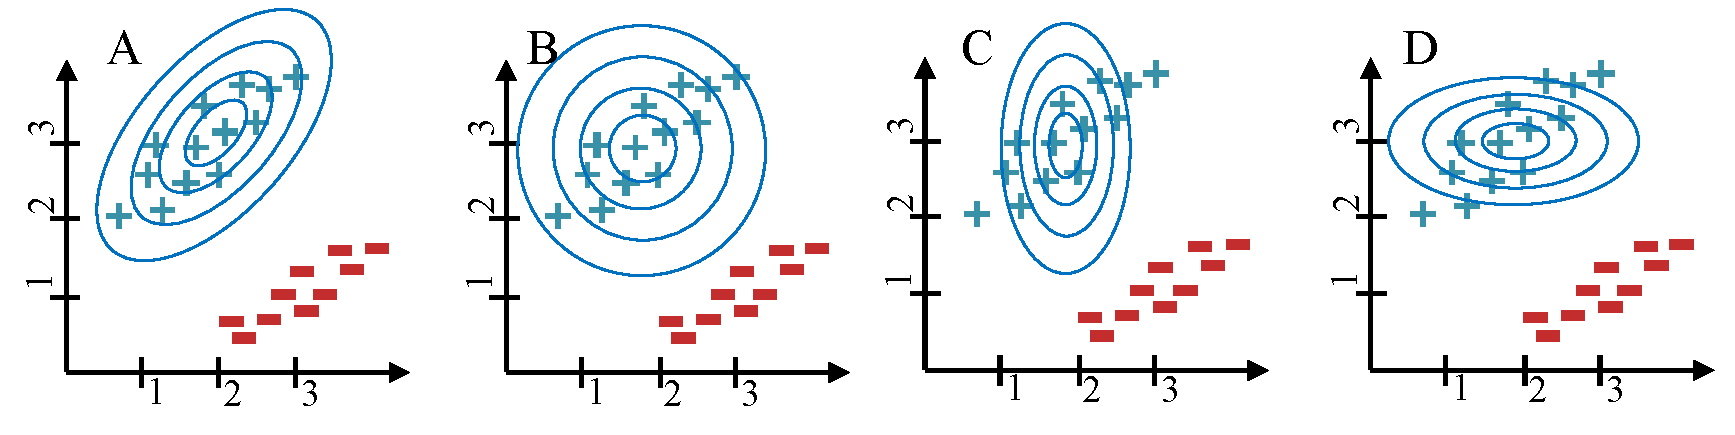
\includegraphics[scale=0.5]{figures/contours.pdf}

%     \begin{subparts}
    
%     \subpart[1] \textbf{Select one:} Assuming the means and variances are all learned without parameter tying or fixing to a constant, which of the contour plots describing the density $f(x_1, x_2 \mid y=1)$ best describes what would be learned?
%     \begin{checkboxes}
%      \choice A
%      \choice B
%      \choice C
%      \choice D
%     \end{checkboxes}
%     \begin{soln}
%     B
%     \end{soln}

%     \subpart[1] \textbf{Select one:} Assuming the means are learned but the variances are fixed to 1.0, , which of the contour plots describing the density $f(x_1, x_2 \mid y=1)$ best describes what would be learned?
%     \begin{checkboxes}
%      \choice A
%      \choice B
%      \choice C
%      \choice D
%     \end{checkboxes}
%     \begin{soln}
%     B
%     \end{soln}

%     \end{subparts}
%     \begin{qauthor}
%     Matt
%     \end{qauthor}

\begin{comment}
\part Mr. Chameleon takes lots of selfies and decides to build a classifier to predict a label $y$ indicating whether he looks more like a flamingo or a brown bear in his latest selfie. He designs two features: $x_1$ stores the \% of pink pixels binned into three bins (0-32, 33-65, 66-100), $x_2$ stores the \% of brown pixels binned into two bins (0-49, 50-100). 

\begin{center}
\begin{tabular}{ccc}
    \toprule
    $x_1$ & $x_2$ & $y$  \\
    \midrule
    66-100 & 0-49 & bear \\
    66-100 & 0-49 & flamingo \\
    33-65 & 0-49 & flamingo \\
    33-65 & 50-100 & bear \\
    0-32 & 50-100 & bear \\
    \bottomrule
\end{tabular}
\end{center}

%The feature design leaves Mr. Chameleon feeling a bit mixed-up, since he can use neither Bernoulli Naive Bayes, nor Multinomial Naive Bayes. He combines the two into a new model, Mixed-up Naive Bayes, that uses a Multinomial event model for $p(x_1 \mid y)$, a Bernoulli event model for $p(x_2 \mid y)$, and a separate Bernoulli for $p(y)$.
The feature design leads Mr. Chameleon to use a Multinomial Naive Bayes model.
%, but he's a bit mixed-up about how to train the model. Help him answer these questions.

    \begin{subparts}

    \subpart[1] \textbf{Numerical answer:} How many parameters does this Multinomial Naive Bayes model have for the given dataset?
        \begin{tcolorbox}[fit,height=1cm, width=2cm, blank, borderline={1pt}{-2pt}]
        %solution
        \end{tcolorbox}
        \begin{soln}
        7 =  4 for $x_1$, 2 for $x_2$, 1 for $y$
        \end{soln}

    \subpart[1] \textbf{Numerical answer:} What is the MLE for $p(y = \text{flamingo})$?
        \begin{tcolorbox}[fit,height=1cm, width=2cm, blank, borderline={1pt}{-2pt}]
        %solution
        \end{tcolorbox}
        \begin{soln}
        2/5
        \end{soln}
    
    \subpart[1] \textbf{Numerical answer:} What is the MLE for $p(x_1 = \text{0-32} \mid y = \text{flamingo})$?
        \begin{tcolorbox}[fit,height=1cm, width=2cm, blank, borderline={1pt}{-2pt}]
        %solution
        \end{tcolorbox}
        \begin{soln}
        0
        \end{soln}
        
    \subpart[1] \textbf{Numerical answer:} What is the MLE for $p(x_1 = \text{0-32} \mid y = \text{bear})$?
        \begin{tcolorbox}[fit,height=1cm, width=2cm, blank, borderline={1pt}{-2pt}]
        %solution
        \end{tcolorbox}
        \begin{soln}
        1/3
        \end{soln}

    \subpart[1] \textbf{Numerical answer:} What is the MLE for $p(x_2 = \text{0-49} \mid y = \text{bear})$?
        \begin{tcolorbox}[fit,height=1cm, width=2cm, blank, borderline={1pt}{-2pt}]
        %solution
        \end{tcolorbox}
        \begin{soln}
        1/3
        \end{soln}
    
    % \uplevel{
    % Suppose Mr. Chameleon collects an additional one hundred training examples and learns the following parameters of the model.

    % \begin{align*}
    %     & p(y = \text{flamingo}) = 3/10 \\
    %     & p(y = \text{bear}) = 7/10 \\
    %     & p(x_1 = \text{0-32} \mid y = \text{flamingo}) = 3/10 \\
    %     & p(x_2 \text{0-49 \mid y = \text{bear}) = 7/10 \\
    % \end{align*}
    
    % }
                
    % \subpart[1] \textbf{Select one:} After completing his maximum likelihood estimation of all the parameters, Mr. Chameleon takes a test selfie and mistakenly\footnote{Kindly ignore Mr. Chameleon's error and proceed with the features he has given, even though they imply a total percentage of pink and brown pixels greater then 100\%.} writes down the following features $x1 = \text{66-100}$ and $x_2 = \text{50-100}$. How would his Mixed-up Naive Bayes model classify this test instance? 
    %     \begin{checkboxes}
    %      \choice flamingo
    %      \choice bear
    %      \choice tie in probability
    %     \end{checkboxes}
    %     \begin{soln}
    %     Both $p(y = \text{flamingo} \mid \xv)$ and $p(y = \text{bear} \mid \xv)$ have zero probability. It's a tie.
    %     \end{soln}

       
    \subpart[2] \textbf{Select one:} After completing his maximum likelihood estimation of all the parameters, Mr. Chameleon takes a test selfie and writes down the features of this test instance as $x_1 = \text{66-100}$ and $x_2 = \text{0-49}$. How would his model classify this test instance? 
        \begin{checkboxes}
         \choice flamingo
         \choice bear
         \choice tie in probability
        \end{checkboxes}
        \begin{soln}
        flamingo: 1/2 * 1/2 * 2/5
        bear: 1/3 * 1/3 * 3/5
        \end{soln}
        
    \end{subparts}
    \begin{qauthor}
    Matt
    \end{qauthor}

\part[1] \textbf{Short answer:} Give one example in which MAP estimation might be preferred over MLE when training a Naive Bayes classifier for classifying whether a document was authored by Henry David Thoreau or Rachel Carson using word counts as features.
    \fillwithlines{6em}
    \begin{soln} 

    If there are words that only appear with one label in the training data, MLE would give zero probability to the other label whenever that word is present, but MAP might not. 

    If you know one author is more inclined to write about one topic than the other author (e.g. marine biology for Rachel Carson and the other about civil disobediance for Henry David Thoreau), imposing a prior over those topic oriented words could help.

    If you don't have much training data, but you have world knowledge about the authors.
    
    Very general answer that is sort of correct, but doesn't address the specific case of Naive Bayes for authorship classification: MAP estimation is preferred over other methods of estimation when there is some prior information available and the amount of available data is limited. It allows us to incorporate this prior information into our estimate. %\\
    %MAP estimation may not be appropriate when the prior information is unreliable or inconsistent with the observed data. 
    \end{soln}
    \begin{qauthor}
    Yash, MLE and MAP
    \end{qauthor}   
\end{comment}
\end{parts}
\clearpage
%\sectionquestion{Miscellaneous}

\begin{parts}

\part[1] \textbf{Short answer:} Describe \textbf{one} topic \textbf{in detail} from the course material \textbf{in Lectures 1--7} that was \textbf{not covered on the exam}, but that you studied thoroughly. For example, a learning objective that you reviewed that was not asked about here, a comparison of two algorithms or ML methods, etc. Write your answer in \textbf{3-5 sentences}.
    \fillwithlines{18em}
    \begin{soln}
    Accept pretty much anything.
    \end{soln}
    \begin{qauthor}
    Matt
    \end{qauthor}
    
\end{parts}
    
% \clearpage
\end{questions}

\clearpage
\begin{center}
Do not remove this page! Use this page for scratch work.
\end{center}
\clearpage
\begin{center}
Do not remove this page! Use this page for scratch work.
\end{center}
\clearpage
\begin{center}
Do not remove this page! Use this page for scratch work.
\end{center}
\clearpage
\begin{center}
Do not remove this page! Use this page for scratch work.
\end{center}

\end{document}
